\documentclass[arguments, manuscript, 11pt]{aastex631}
\makeatletter
\let\frontmatter@title@above=\relax
\makeatother

% Horizontal lines
\newcommand{\HRule}{\rule{\linewidth}{0.5mm}}
\newcommand*{\threeemdash}{\rule[0.5ex]{30em}{0.55pt}}


\usepackage{lipsum}% for placeholder text
 \usepackage{booktabs}
  \usepackage{multirow}
\usepackage{graphicx}
\usepackage[bottom]{footmisc}
\usepackage{setspace}
\renewcommand{\footnotelayout}{\setstretch{0.75}}

\raggedbottom

\doublehyphendemerits=10000 % No consecutive line hyphens
\brokenpenalty=10000 % No broken words across columns/pages
\widowpenalty=9999 % Almost no widows at bottom of page
\clubpenalty=9999 % Almost no orphans at top of page
\interfootnotelinepenalty=9999 % Almost never break footnotes

% Math symbols
\usepackage{amssymb,amsfonts,mathtools} % Math Symbols
\usepackage{amsmath} % Symbols
\newtheorem{assumption}{Assumption} %Assumption
\usepackage{textgreek} % Greek letters
\usepackage{xfrac} %Fractions
\usepackage{units} %Diagonal fraction
\usepackage[official]{eurosym} % Euro symbol
\usepackage{breqn} % For some weird equations
\usepackage{textcomp} %Needed for the per mile symbol
\usepackage{bbm} % For the indicator function

% argmin argmax
\DeclareMathOperator*{\argmax}{arg\,max}
\DeclareMathOperator*{\argmin}{arg\,min}


%% where the layout options are:
%%
%%  twocolumn   : two text columns, 10 point font, single spaced article.
%%                This is the most compact and represent the final published
%%                derived PDF copy of the accepted manuscript from the publisher
%%  manuscript  : one text column, 12 point font, double spaced article.
%%  preprint    : one text column, 12 point font, single spaced article.  
%%  preprint2   : two text columns, 12 point font, single spaced article.
%%  modern      : a stylish, single text column, 12 point font, article with
%% 		  wider left and right margins. This uses the Daniel
%% 		  Foreman-Mackey and David Hogg design.
%%  RNAAS       : Supresses an abstract. Originally for RNAAS manuscripts 
%%                but now that abstracts are required this is obsolete for
%%                AAS Journals. Authors might need it for other reasons. DO NOT
%%                use \begin{abstract} and \end{abstract} with this style.
%%
%% Note that you can submit to the AAS Journals in any of these 6 styles.
%%
%% There are other optional arguments one can invoke to allow other stylistic
%% actions. The available options are:
%%
%%   astrosymb    : Loads Astrosymb font and define \astrocommands. 
%%   tighten      : Makes baselineskip slightly smaller, only works with 
%%                  the twocolumn substyle.
%%   times        : uses times font instead of the default
%%   linenumbers  : turn on lineno package.
%%   longauthor   : Do not use the more compressed footnote style (default) for 
%%                  the author/collaboration/affiliations. Instead print all
%%                  affiliation information after each name. Creates a much 
%%                  longer author list but may be desirable for short 
%%                  author papers.
%% twocolappendix : make 2 column appendix.
%%   anonymous    : Do not show the authors, affiliations and acknowledgments 
%%                  for dual anonymous review.
%%
%% these can be used in any combination, e.g.
%%
%% \documentclass[twocolumn,linenumbers]{aastex631}
%%
%% AASTeX v6.* now includes \hyperref support. While we have built in specific
%% defaults into the classfile you can manually override them with the
 %%\hypersetup 
%%
\hypersetup{linkcolor=red,citecolor=blue,filecolor=cyan,urlcolor=magenta}
%% will change the color of the internal links to red, the links to the
%% bibliography to green, the file links to cyan, and the external links to
%% magenta. Additional information on \hyperref options can be found here:
%% https://www.tug.org/applications/hyperref/manual.html#x1-40003
%%
%% Note that in v6.3 "bookmarks" has been changed to "true" in hyperref
%% to improve the accessibility of the compiled pdf file.
%%
%% If you want to create your own macros, you can do so
%% using \newcommand. Your macros should appear before
%% the \begin{document} command.
%%
\newcommand{\vdag}{(v)^\dagger}
\newcommand\aastex{AAS\TeX}
\newcommand\latex{La\TeX}

%% Reintroduced the \received and \accepted commands from AASTeX v5.2
%%\received{March 1, 2021}
%%\accepted{\today}
%%\date{\today}
%% Command to document which AAS Journal the manuscript was submitted to.
%% Adds "Submitted to " the argument.
%%\submitjournal{PSJ}

%% For manuscript that include authors in collaborations, AASTeX v6.31
%% builds on the \collaboration command to allow greater freedom to 
%% keep the traditional author+affiliation information but only show
%% subsets. The \collaboration command now must appear AFTER the group
%% of authors in the collaboration and it takes TWO arguments. The last
%% is still the collaboration identifier. The text given in this
%% argument is what will be shown in the manuscript. The first argument
%% is the number of author above the \collaboration command to show with
%% the collaboration text. If there are authors that are not part of any
%% collaboration the \nocollaboration command is used. This command takes
%% one argument which is also the number of authors above to show. A
%% dashed line is shown to indicate no collaboration. This example manuscript
%% shows how these commands work to display specific set of authors 
%% on the front page.
%%
%% For manuscript without any need to use \collaboration the 
%% \AuthorCollaborationLimit command from v6.2 can still be used to 
%% show a subset of authors.
%
%\AuthorCollaborationLimit=2
%
%% will only show Schwarz & Muench on the front page of the manuscript
%% (assuming the \collaboration and \nocollaboration commands are
%% commented out).
%%
%% Note that all of the author will be shown in the published article.
%% This feature is meant to be used prior to acceptance to make the
%% front end of a long author article more manageable. Please do not use
%% this functionality for manuscripts with less than 20 authors. Conversely,
%% please do use this when the number of authors exceeds 40.
%%
%% Use \allauthors at the manuscript end to show the full author list.
%% This command should only be used with \AuthorCollaborationLimit is used.

%% The following command can be used to set the latex table counters.  It
%% is needed in this document because it uses a mix of latex tabular and
%% AASTeX deluxetables.  In general it should not be needed.
\setcounter{table}{0}

%%%%%%%%%%%%%%%%%%%%%%%%%%%%%%%%%%%%%%%%%%%%%%%%%%%%%%%%%%%%%%%%%%%%%%%%%%%%%%%%
%%
%% The following section outlines numerous optional output that
%% can be displayed in the front matter or as running meta-data.
%%
%% If you wish, you may supply running head information, although
%% this information may be modified by the editorial offices.
%\shorttitle{AASTeX v6.3.1 Sample article}
\shortauthors{\small Martínez-Jiménez et al. (2025)}
%%
%% You can add a light gray and diagonal water-mark to the first page 
%% with this command:
%%\watermark{DRAFT}
%% where "text", e.g. DRAFT, is the text to appear.  If the text is 
%% long you can control the water-mark size with:
%% \setwatermarkfontsize{1pt}
%% where dimension is any recognized LaTeX dimension, e.g. pt, in, etc.
%%
%%%%%%%%%%%%%%%%%%%%%%%%%%%%%%%%%%%%%%%%%%%%%%%%%%%%%%%%%%%%%%%%%%%%%%%%%%%%%%%%
\graphicspath{{../FIGURES/}{../Figures/}{./}{FIGURES/}{figures/}}
%% This is the end of the preamble.  Indicate the beginning of the
%% manuscript itself with \begin{document}.
\usepackage[english]{babel}
\usepackage[autostyle]{csquotes}

\usepackage{changepage}

\newcommand{\firstpageruleack}[1]{%
  \par\vspace*{\fill}%
\noindent\hspace*{2em}\rule{0.8\linewidth}{0.4pt}
  \par\vspace{0.4em}%
  {\scriptsize #1\par}%
  \thispagestyle{empty}%
  \clearpage
}
\begin{document}
\vspace{-1.5in} 

\title{
\phantom{hhhhhhh} \\ \phantom{hhhhhhh} \\ \Large How Do Economic Shocks Impact Upon the \\Mental Health of Retirees? \\[8pt]}

%% LaTeX will automatically break titles if they run longer than
%% one line. However, you may use \\ to force a line break if
%% you desire. In v6.31 you can include a footnote in the title.

%% A significant change from earlier AASTEX versions is in the structure for 
%% calling author and affiliations. The change was necessary to implement 
%% auto-indexing of affiliations which prior was a manual process that could 
%% easily be tedious in large author manuscripts.
%%
%% The \author command is the same as before except it now takes an optional
%% argument which is the 16 digit ORCID. The syntax is:
%% \author[xxxx-xxxx-xxxx-xxxx]{Author Name}
%%
%% This will hyperlink the author name to the author's ORCID page. Note that
%% during compilation, LaTeX will do some limited checking of the format of
%% the ID to make sure it is valid. If the "orcid-ID.png" image file is 
%% present or in the LaTeX pathway, the OrcID icon will appear next to
%% the authors name.
%%
%% Use \affiliation for affiliation information. The old \affil is now aliased
%% to \affiliation. AASTeX v6.31 will automatically index these in the header.
%% When a duplicate is found its index will be the same as its previous entry.
%%
%% Note that \altaffilmark and \altaffiltext have been removed and thus 
%% can not be used to document secondary affiliations. If they are used latex
%% will issue a specific error message and quit. Please use multiple 
%% \affiliation calls for to document more than one affiliation.
%%
%% The new \altaffiliation can be used to indicate some secondary information
%% such as fellowships. This command produces a non-numeric footnote that is
%% set away from the numeric \affiliation footnotes.  NOTE that if an
%% \altaffiliation command is used it must come BEFORE the \affiliation call,
%% right after the \author command, in order to place the footnotes in
%% the proper location.
%%
%% Use \email to set provide email addresses. Each \email will appear on its
%% own line so you can put multiple email address in one \email call. A new
%% \correspondingauthor command is available in V6.31 to identify the
%% corresponding author of the manuscript. It is the author's responsibility
%% to make sure this name is also in the author list.
%%
%% While authors can be grouped inside the same \author and \affiliation
%% commands it is better to have a single author for each. This allows for
%% one to exploit all the new benefits and should make book-keeping easier.
%%
%% If done correctly the peer review system will be able to
%% automatically put the author and affiliation information from the manuscript
%% and save the corresponding author the trouble of entering it by hand.

%\correspondingauthor{Mario Martínez-Jiménez, Imperial College Business School, London SW7 2AZ, United Kingdom}
%\email{m.martinez-jimenez@imperial.ac.uk}
\vspace{1cm}
\author[0000-0001-6189-6494]{Mario Martínez-Jiménez}
\affiliation{Department of Health Policy, Stanford University, Stanford, California, United States of America}
\affiliation{Department of Economics \& Public Policy, Imperial Business School, London, United Kingdom}
\affiliation{Centre for Health Economics \& Policy Innovation, Imperial Business School, London, United Kingdom}

\author[0000-0002-4314-6523]{Bruce Hollingsworth}
\affiliation{Division of Health Research, Lancaster University, Lancaster, United Kingdom}

\author[0000-0003-3883-5006]{Eugenio Zucchelli}
\affiliation{Department of Economic Analysis, Universidad Autónoma de Madrid (UAM), Spain}
\affiliation{Lancaster University, United Kingdom}
\affiliation{IZA, Germany}








%% Note that the \and command from previous versions of AASTeX is now
%% depreciated in this version as it is no longer necessary. AASTeX 
%% automatically takes care of all commas and "and"s between authors names.

%% AASTeX 6.31 has the new \collaboration and \nocollaboration commands to
%% provide the collaboration status of a group of authors. These commands 
%% can be used either before or after the list of corresponding authors. The
%% argument for \collaboration is the collaboration identifier. Authors are
%% encouraged to surround collaboration identifiers with ()s. The 
%% \nocollaboration command takes no argument and exists to indicate that
%% the nearby authors are not part of surrounding collaborations.

%% Mark off the abstract in the ``abstract'' environment. 

\begin{abstract}
\linespread{0.85} 

\noindent\begin{minipage}{0.85\textwidth}
\vspace{0.5cm}
\footnotesize{Economic crises may alter how retirement affects mental health. This paper studies whether the mental health consequences of retirement differ when older workers retire in region-years more exposed to the Great Recession. Using longitudinal data from the English Longitudinal Study of Ageing (ELSA) for 2002--2019, we estimate fixed-effects and instrumental-variables fixed-effects models that exploit the statutory pension age and its interaction with local crisis intensity. We focus on two mental health outcomes: a binary depression indicator based on the eight-item CES-D scale and a new psychiatric diagnosis indicator. In the short run (2009--2013), retirement in high-unemployment region-years is associated with a 5.1 percentage point reduction in the probability of reporting a new psychiatric diagnosis, while evidence for the depression indicator is weaker and points in the opposite direction. In the longer run (2009--2019), the short-run decline in psychiatric diagnoses does not persist, and retirement in harder-hit regions is associated with higher depression prevalence. These results suggest that macroeconomic conditions shape the mental health consequences of retirement and that short-run relief from clinical diagnoses need not translate into broader or lasting improvements in depressive symptoms.}\\
\vspace{-0.25cm}\\
\noindent\textbf{Keywords:} retirement; mental health; depression; economic shocks; causal inference\\
\noindent\textbf{JEL Codes:} J14; J26; I10\\
\end{minipage}

\firstpageruleack{\\
Corresponding author: \emph{Mario Martínez-Jiménez}. Email: \texttt{mmarjim3@stanford.edu}. 
\\
 We would like to thank the UK Data Service for providing the data. We thank participants at the 2020 UK Health Economist's Study Group (HESG) winter meeting in Newcastle, the 2021 LolaHESG (lowlands Health Economic Study Group) conference and attendants to seminars at Lancaster University, UK, and the PHE Public Health Research and Science Conference 2021, for valuable comments. We also would like to thank Katharina Janke and members of the Health Economics at Lancaster (HEAL) research group for their useful suggestions. This work was supported by the NIHR School of Public Health Research (SPHR), Liverpool and Lancaster Collaboration for Public Health Research (LiLaC). One of the authors acknowledges funding from the Spanish Ministry of Science, Innovation and Universities (Grant PID2022-137819NB-I00). 
%\vspace{5cm}
}
\end{abstract}

%% Keywords should appear after the \end{abstract} command. 
%% The AAS Journals now uses Unified Astronomy Thesaurus concepts:
%% https://astrothesaurus.org
%% You will be asked to selected these concepts during the submission process
%% but this old "keyword" functionality is maintained in case authors want
%% to include these concepts in their preprints.




%% From the front matter, we move on to the body of the paper.
%% Sections are demarcated by \section and \subsection, respectively.
%% Observe the use of the LaTeX \label
%% command after the \subsection to give a symbolic KEY to the
%% subsection for cross-referencing in a \ref command.
%% You can use LaTeX's \ref and \label commands to keep track of
%% cross-references to sections, equations, tables, and figures.
%% That way, if you change the order of any elements, LaTeX will
%% automatically renumber them.
%%
%% We recommend that authors also use the natbib \citep
%% and \citet commands to identify citations.  The citations are
%% tied to the reference list via symbolic KEYs. The KEY corresponds
%% to the KEY in the \bibitem in the reference list below. 
\setcounter{page}{0}
\thispagestyle{empty}
\pagebreak 

\newpage


\section{Introduction} \label{sec:introduction}

The population in high-income countries is ageing rapidly. In 2014, 17.6\% of the UK population was aged 65 or older, rising to 19\% by 2022 and projected to rise further in the coming decades \citep{park2023population}. Older adults often face health challenges and major life transitions that heighten their risk of mental health problems \citep{national2018healthy}. A growing literature studies the health effects of retirement (e.g., \cite{bonsang2012retirement}; \cite{eibich2015understanding}; \cite{fitzpatrick2018mortality}; \cite{ebeid2023short}), but findings remain mixed across settings, methodologies, and outcomes. One reason is that the mental health effect of retirement may depend on the macroeconomic environment in which retirement occurs.

This paper examines whether the effect of retirement on mental health differs in the presence of economic shocks, highlighting the importance of understanding which socioeconomic factors moderate this relationship. This is relevant in policy terms, especially in the light of devising policies aimed at retaining an ageing workforce. Previous literature on the impact of economic shocks on health also presents varying and inconclusive results (e.g., \cite{di2001preferences}; \cite{modrek2013review}; \cite{karanikolos2013financial}). \cite{ruhm2000recessions} seminal work on the effects of macroeconomic conditions on health shows that in the US mortality appears to be procyclical and this is confirmed by other studies using data from different countries, including Spain \citep{granados2005recessions}; Germany \citep{neumayer2004recessions}; France \citep{buchmueller2007unemployment}; Canada \citep{ariizumi2012recessions}; and Mexico \citep{gonzalez2011macroeconomic}. However, a more recent strand of the literature finds that mortality is either countercyclical or unaffected by macroeconomic shocks (\cite{ruhm2015recessions}; \cite{tekin2013health}). The inconsistent findings in the retirement--health literature may partly reflect differences in economic conditions at the time of retirement. In this paper, we study whether regional economic shocks during the Great Recession provide a plausible explanation for the heterogeneous effects reported in earlier studies.

This paper asks whether the mental health effect of retirement changes during a severe economic downturn. Using longitudinal data from eight waves (2002--2019) of the English Longitudinal Study of Ageing (ELSA), we combine regional variation in unemployment during and after the Great Recession with panel methods that absorb time-invariant individual heterogeneity. To address endogeneity in retirement timing, we estimate instrumental-variables fixed-effects models that exploit the statutory pension age and its interaction with crisis exposure. We focus on two mental health outcomes: a binary depression indicator defined as reporting four or more symptoms on the eight-item CES-D scale, and a new psychiatric diagnosis indicator. We interpret the continuous CES-D count as an alternative outcome and report it in the appendix.

Our findings point to a more nuanced mental health pattern than a simple ``retirement improves mental health during crises'' interpretation. In the short run, retirement in harder-hit region-years is associated with a lower probability of reporting a new psychiatric diagnosis, but the same interaction does not deliver broader improvement in depressive symptoms. In the longer run, the short-run reduction in psychiatric diagnoses disappears, while the depression indicator increases in high-unemployment region-years. Subgroup estimates suggest that the short-run decline in psychiatric diagnoses is concentrated among men and white-collar workers, but these heterogeneous patterns are less precisely estimated than the main all-sample results and are interpreted cautiously.

This paper offers three contributions. First, it provides new evidence on how the mental health consequences of retirement vary with local exposure to a major macroeconomic shock. Second, it studies England, where private pension exposure and labour-market conditions make the Great Recession a particularly informative setting for the retirement--mental-health relationship. Third, it distinguishes between clinically reported psychiatric diagnoses and a broader depression-symptom indicator, showing that these outcomes need not move together. This distinction is important for policy because it suggests that short-run relief from clinical diagnoses may coexist with later deterioration in broader depressive symptoms.

Secondly, our study highlights England, an economy severely impacted by its financial system during this time. The UK's pension system heavily relies on private pension schemes linked to financial markets, making retirees more vulnerable to economic downturns. Compared to countries with larger state pension systems, such as France or Germany, where public pensions form the primary source of retirement income, the UK's approach involves a significant degree of market exposure and investment risk. This reliance on market-dependent pensions amplifies the financial strain on retirees during recessions, offering a unique context to assess the health impacts of retirement in economic crises. 

Thirdly, our longitudinal data enable us to emphasise the circumstances that influence the relationship between mental health, retirement, and economic shocks. To the best of our knowledge, no prior study has examined this relationship within the context of England, nor has it highlighted the financial, social, and behavioural determinants of this phenomenon. Our findings emphasise the significance of financial stability, healthy lifestyles, and timely retirement in achieving the mental health benefits of retirement amidst economic crises. These insights are crucial for developing focused retirement and social support policies, especially for economically vulnerable regions.


\section{Background} \label{sec:background}
\subsection{Related Literature} \label{sec:literature}
Empirical studies on the causal impact of retirement on health often present conflicting results. This might be due to differences in the methods and data used as well as the varying institutional incentives or ability to retire across different countries. More specifically, studies using an instrumental variable (IV) approach (often exploiting statutory retirement age) tend to find positive impacts of retirement on health (e.g., \cite{bound2007estimating}; \cite{neuman2008quit}; \cite{bonsang2012retirement}), whereas studies employing panel data methods tend to find negative effects (e.g., \cite{dave2006effects}; \cite{bamia2007age}). 

\cite{gorry2018does} use eligibility for social security as an instrument for retirement on US data from the Health and Retirement Study and find that retirement improves self-reported health and mental health. Results from Coe and Zamarro (2011) obtained by exploiting country-specific early and full retirement ages as instruments for retirement and data from SHARE suggest no significant effects of retirement on health. \cite{eibich2015understanding} and \cite{rose2020retirement} use a Regression Discontinuity Design (RDD) based on financial incentives in the German and English pension systems, respectively. Both studies find that retirement improves subjective health status. Studies evaluating the effects of changes to the State Pension age on health also report mixed results. \cite{ebeid2023short}, using a nonparametric fuzzy RDD, find that retirement has a negative effect on cognitive function and depression symptoms in the short term. Recently, \cite{carrino2020later} used data from Understanding Society between 2009-2016 and the raising of the state pension age among women as an instrument. They find that raising the state pension age leads to a decline in mental health among women in lower occupational groups.\footnote{Other studies evaluating the effects of lowering the State Pension age report either negative effects \citep{bloemen2017causal} or no effects on mortality \citep{hernaes2013does}.}

Estimates on the impact of labour market status on health during economic shocks are also inconsistent (\cite{browning2012effect}; \cite{avdic2021economic}). A strand of studies finds that economic shocks can negatively affect health outcomes by increasing the stress associated with job loss and reducing monetary and non-monetary benefits (e.g., by reducing the availability of flexible time, periods of leave, mentoring and childcare-related programs) and that these effects vary by age, sex and occupational status (e.g. \cite{eliason2009does}; \cite{sullivan2009job}; \cite{jofre2018impact}; \cite{black2022whose}). Previous literature has so far paid less attention to the impact of economic shocks on the health of older individuals. \cite{mcinerney2012recessions} estimate that during economic shocks, the mental health of older individuals appears to deteriorate and that such individuals are also less likely to engage in healthy behaviours. \cite{ruhm2002does} also find that older individuals tend to engage less in potentially risky behaviours during periods of recessions. Overall, this indicates that the health effects associated with retirement may vary according to the macroeconomic conditions present at the time of retirement.

However, some individuals are more protected from these risks due to differences in occupational status. In particular, white-collar workers are often shielded from financial uncertainty as they near retirement because their pension funds are typically de-risked in the years leading up to retirement, with investments shifting from equities to lower-risk assets such as bonds or cash. This transition helps protect their pension savings from stock market downturns, ensuring that an economic shock does not directly impact their retirement income. In contrast, those in lower-paid or precarious jobs may have less access to such structured pension protections, rendering them more vulnerable to financial instability and its associated health risks as they approach retirement. This paper examines whether the effects of retirement and economic shocks on older individuals' health differ depending on key moderators.



\subsection{Economic shocks, retirement and health} \label{sec:model}

Standard models of health investment (\cite{grossman1972concept}; \cite{grossman2000human}) suggest that while the depreciation rate on an individual’s health stock increases with age, individuals would still invest in their own health. For instance, individuals may still invest in their health capital post-retirement, even though this will no longer increase their labour productivity or earnings, as “healthy time” also enters the utility function directly as a consumption good \citep{dave2006effects}. According to this interpretation, the direction of the effect of retirement on health is ambiguous and would also depend on the marginal value of time after retirement.

At older ages, mental health is shaped not only by physical and social environments but also by experiencing stressful events, such as retirement \citep{minkler1981research}. Several studies suggest that changes in labour market conditions may affect health by increasing psychological distress from income and wealth shocks \citep{black2022whose}. Therefore, it is plausible that retiring during or immediately after an economic downturn could improve mental health by alleviating job-related strain. However, economic crises frequently result in decreased pensions, diminished savings, and rising living expenses, worsening financial insecurity for retirees with limited savings. Importantly, the extent of financial vulnerability in retirement depends on occupational status and the structure of pension schemes. In the UK, where market-linked pensions play a significant role, those in lower-paid or precarious jobs may be more exposed to financial instability, as their pension savings may depreciate with inflation. In contrast, many white-collar workers benefit from automatic pension de-risking, where funds shift to lower-risk assets such as bonds or cash in the years leading up to retirement, shielding their savings from stock market shocks. Compared to countries such as France and Germany, where public pensions provide a more stable income base, the UK's system may leave certain groups more vulnerable. The uncertainty that accompanies economic downturns can also heighten feelings of anxiety and depression, particularly among those who struggle to maintain healthy coping strategies in retirement.

To the best of our knowledge, the study by \cite{belloni2016effect} is the only one attempting to estimate the impact of retirement on health while accounting for the geographical differences in the intensity of the economic crisis in European countries. They find that retiring immediately after an economic shock improves mental health, although only among blue-collar men living in the most severely affected regions. While their findings highlight important heterogeneity in the retirement--mental health relationship by occupation and local crisis intensity, the study does not examine whether financial, social, or behavioural factors moderate these effects. In particular, blue-collar workers may need to retire later than the state pension age due to financial constraints, whereas white-collar workers can often retire earlier due to their private pensions, potentially influencing the observed health effects of retirement. Our analysis differs from this paper by focusing on the actual age at which these population subgroups retire during the same macroeconomic shock while providing insights into the longer-term effects of retirement on health during an economic crisis.

\section{Data} \label{sec:data}

The English Longitudinal Study of Ageing (ELSA) provides rich individual-level health and socioeconomic data from a representative sample of the English population aged 50 and older, collected between March 2002 and July 2019; see Appendix A, Tables A1--A2 for details. The dataset contains detailed information on mental health, employment, wealth, pensions, and local area conditions.

We focus on a group of individuals employed during the first wave (March 2002 – March 2003). Our starting sample comprises employees or self-employed individuals who were engaged in ‘work’ or ‘paid work during the last month’ in this first wave. We exclude those who, despite being classified as ‘in paid work’, also identify as ‘retired’, ‘caring for home or family’, ‘semi-retired’, ‘unemployed’, or ‘disabled’. Our analysis focuses on retirement occurring between consecutive waves, which we define as dependent on employment in the previous wave. Retiree individuals will classify themselves as ‘retired’ and ‘not in work during the last month’ in the subsequent wave. We consider only the initial exits from the labour market and, therefore, perceive retirement as an “absorbing state." Consequently, our retirement variable is a binary indicator, marked as 1 if the individual retires between waves and 0 if still employed between consecutive waves. The main analysis uses an unbalanced sample, with 2,638 individuals; refer to Appendix A, Tables A3--A4 for more details.

Attrition in the English Longitudinal Study of Ageing may be a matter of concern if it affects mental health through sample selection bias. If the likelihood of respondents participating in the survey is negatively related to their mental health, this can skew the retention rate based on our variable of interest. To assess selective attrition, we follow the methodology proposed by \cite{lindeboom2002econometric} and perform two informal tests. The first test relates new psychiatric diagnosis to an attrition dummy (coded as 1 if the respondent is absent from the panel for any wave), the retirement dummy, and several control variables, including individual fixed effects. The findings indicate that neither the attrition dummy nor its interaction with retirement is statistically significant. In the second test, we regress the attrition dummy on new psychiatric diagnosis, again controlling for additional variables and individual fixed effects, and find no significant relationship. This suggests that those experiencing a decline in mental health are not more likely to exit the panel. More details can be found in Appendix A, Table A5.

\subsection{Health outcomes and other key variables} \label{sec:literature}

We focus on mental health outcomes, which are likely to respond more quickly than physical health to the transition out of work \citep{fleischmann2020mental}. Our first outcome is a binary depression indicator based on the 8-item Centre for Epidemiological Studies Depression Scale (CES-D): it equals one when respondents report four or more symptoms and zero otherwise. The underlying symptom count ranges from 0 to 8 and is reported as an alternative outcome in Appendix C. Our second outcome is a new psychiatric diagnosis indicator, which captures whether the respondent reports a new depression or anxiety diagnosis after retirement. This diagnosis measure helps distinguish new onset conditions from persistent pre-retirement mental health problems, although it may still understate prevalence if respondents do not report diagnoses during the interview.\footnote{The diagnosis measure may still underestimate prevalence because some individuals may not report their condition during face-to-face interviews.}

Our analysis controls for a variety of characteristics at the individual, household, and regional levels. These include age, gender, marital status (whether individuals are married or cohabiting), household size (which encompasses both children and adults), outright homeownership, and educational attainment based on the International Standard Classification of Education (ISCED). In terms of pension characteristics, we focus on private pension scheme membership, the total state pension income (measured in pounds per week), and the statutory pension age. We also assess health behaviours by determining whether individuals are current smokers, whether they engage in vigorous or moderate physical activities less than once a week, and if they have health insurance. Moreover, we consider geographical factors, such as area-level deprivation quintiles derived from a multiple deprivation index and population density quintiles based on postcode.

Our mechanisms analysis identifies four key risk factors that may influence the relationship between retirement, health, and economic shocks. First, we consider self-reported net financial wealth, which includes savings and investments, and subtract financial debt, measured at the benefit unit level. For our analysis, we create a binary variable that indicates whether an individual falls into the top quartile of this measure. Second, we measure social isolation by determining if an individual lives with more than one person (including both children and adults) in their household. Third, we evaluate physical activity levels to assess healthy behaviours. This variable assigns a score of one if the respondent engages in moderate or vigorous physical activity and a score of zero if they have low levels of activity.\footnote{We categorise physical activity into three levels: vigorous-intensity (such as running, swimming, cycling, intense aerobics, tennis, and digging), moderate-intensity (like gardening, car cleaning, walking at a moderate pace, and dancing), and low-intensity (including laundry and home repairs). The levels are defined as follows: inactive; engaging in only light activities at least once a week (excluding moderate or vigorous activities); participating in moderate activities at least once weekly (but not vigorous); and performing vigorous activities at least once a week.} Finally, we generate a variable that captures the respondent's age at retirement, specifically identifying individuals who retire before reaching their state pension age.

\subsection{Statutory pension eligibility and intensity of economic crisis } \label{sec:SPA}

From 2002 to 2019, the eligibility rules for state pensions in the UK saw considerable changes for both men and women. Men maintained a state pension age of 65 until 2019, while women’s SPA started at 60 in 2002 and gradually increased from April 2010, reaching 65 by November 2018 to equalise with men. After this adjustment, both men and women saw their SPA rise to 66 by October 2019. These changes were prompted by the Pensions Act 1995 and were expedited by the Pensions Act 2011, which aimed to equalise and elevate the SPA faster than initially intended.\footnote{More information regarding state pension eligibility and rules can be found at \url{https://www.gov.uk/government/publications/your-new-state-pension-explained/your-state-pension-explained}.} Our analysis accounts for these alterations in the eligibility rules for women.

\begin{figure}[htb!]\caption{Retirement age distribution, state pension age eligibility: 2004–2019, men and women}
\begin{center}
\label{fig1}
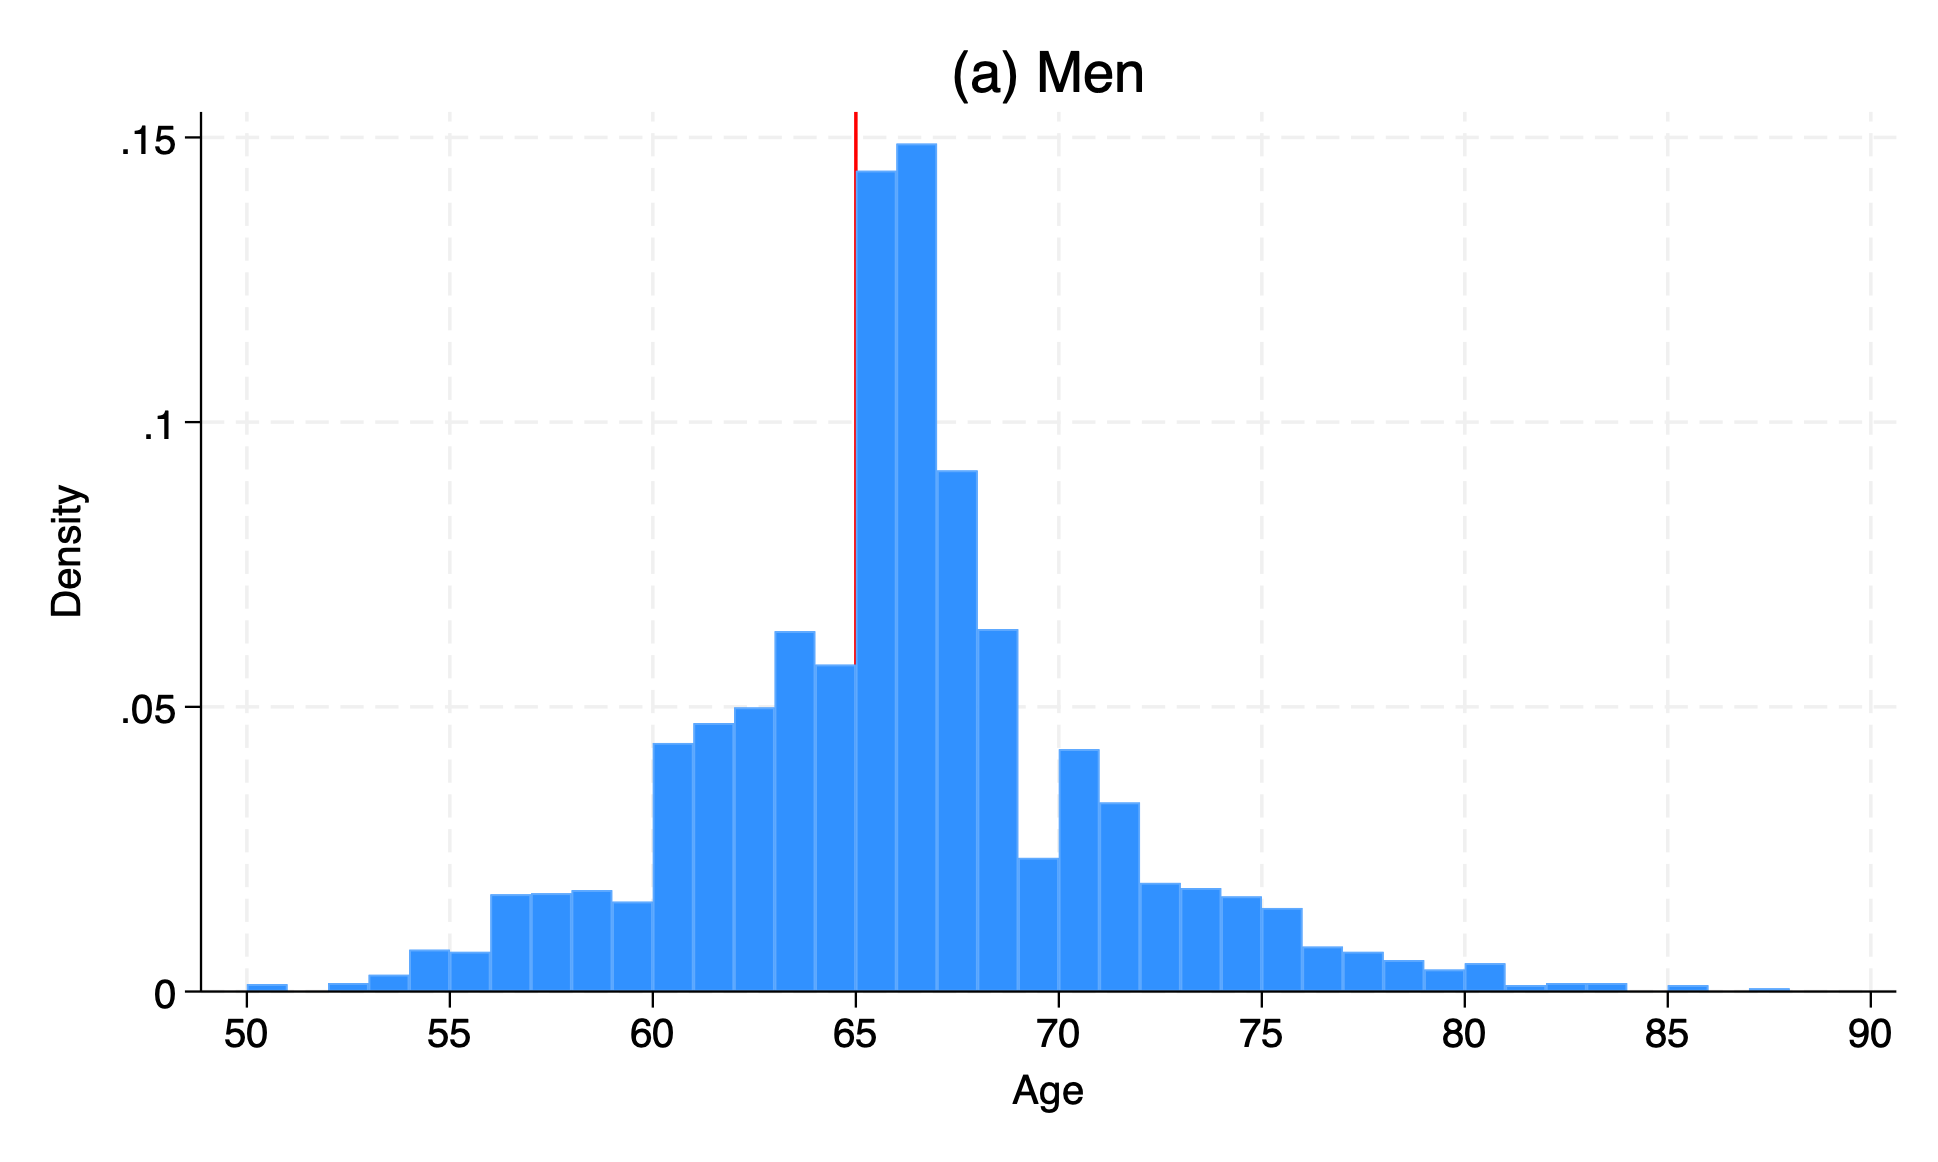
\includegraphics[width=0.725\textwidth]{male.png}
%\hspace{\fill}
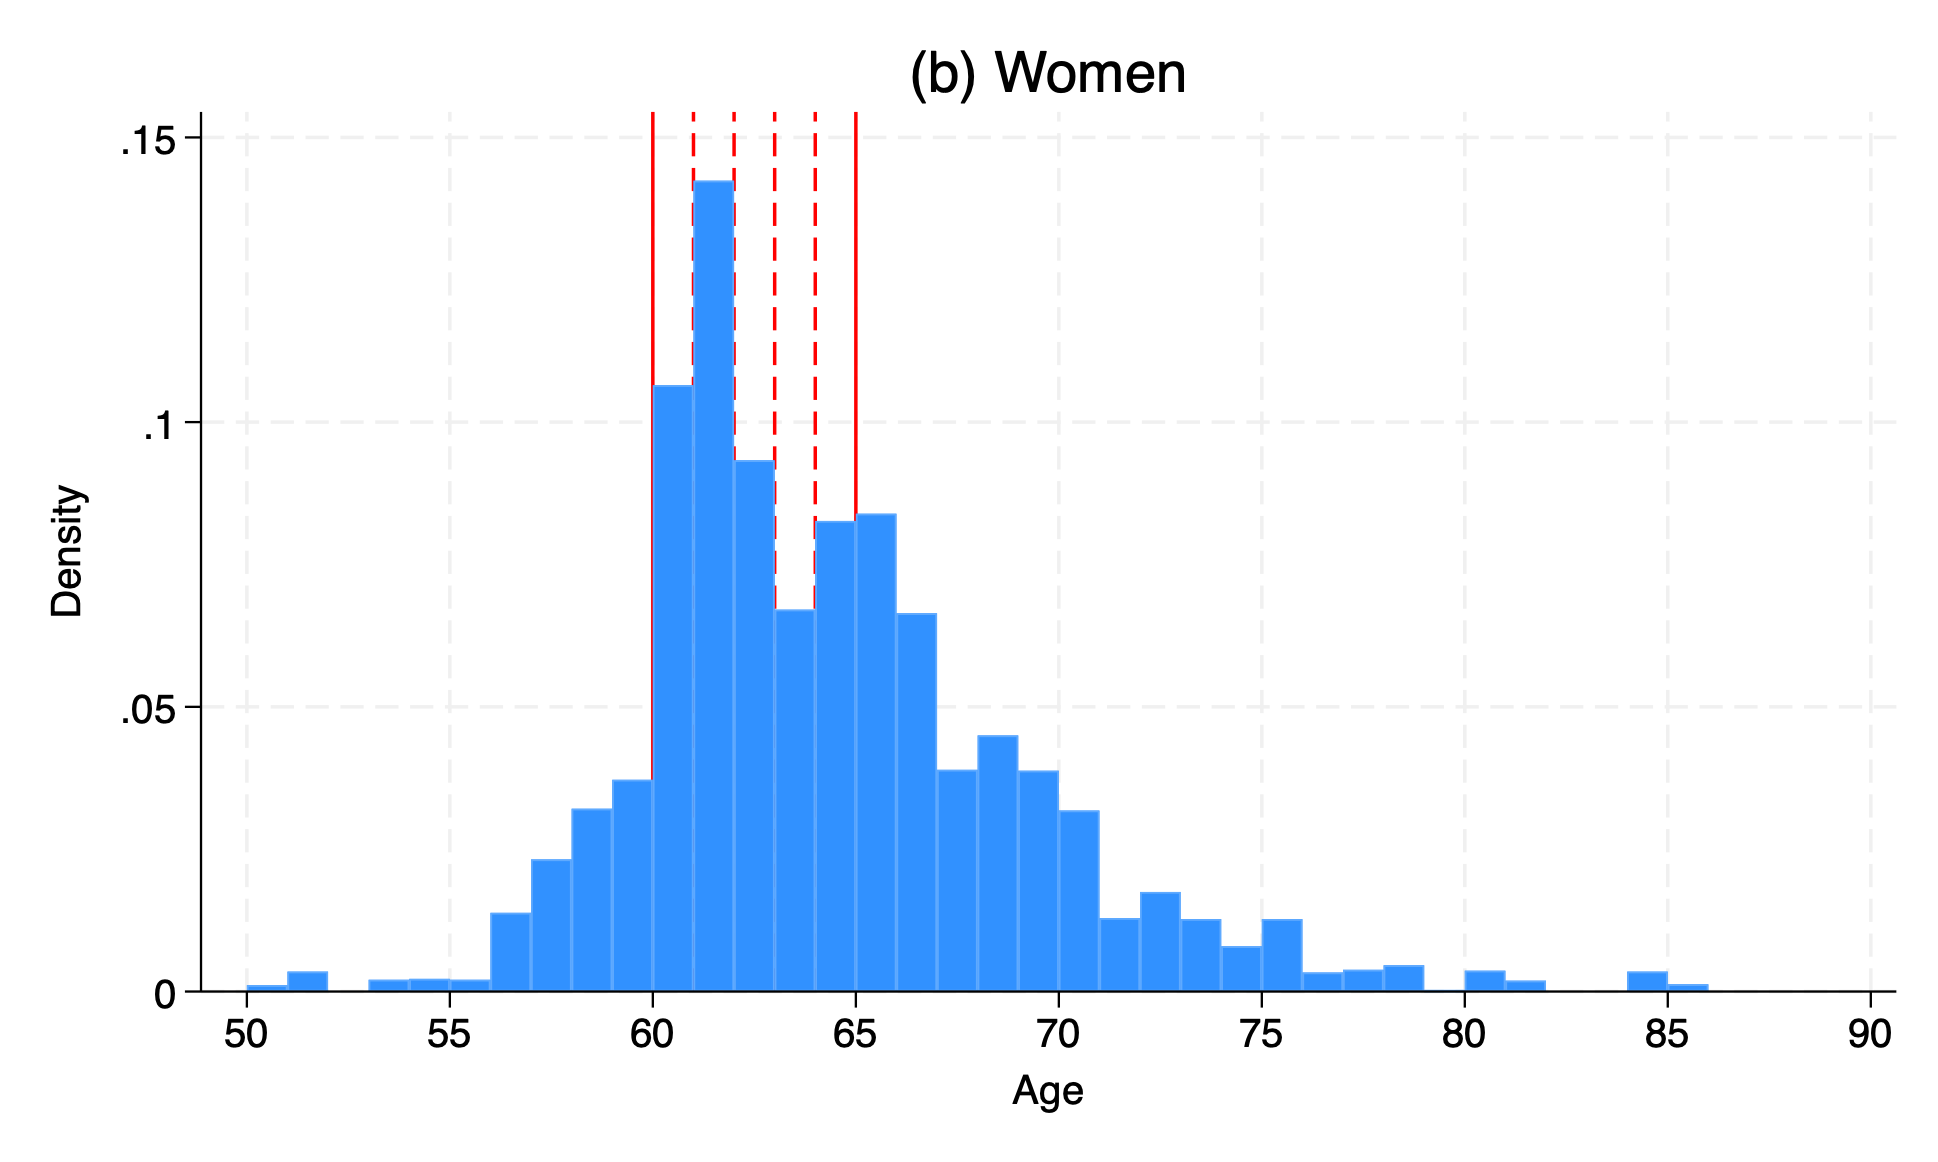
\includegraphics[width=0.725\textwidth]{female.png}
\end{center}
 \vspace*{-1cm}
 
 \scriptsize {\singlespacing \emph{Notes:} Retirement age is computed by exploiting information on the self-reported retirement status and age. From 2004–2009, women's retirement age stayed at 60. From April 2010 to November 2018: it gradually rose from 60 to 65. In 2019, it further increased to 66, fully aligning with men. From 2004 to 2018: Men's State Pension age held steady at 65. A gradual increase occurred from 2018 to 2019, raising it to 66.}
\end{figure}
  
In terms of macroeconomic conditions, we use the annual unemployment rate within each Government Office Region (GOR), the highest tier of the subnational geographical division of England. The Office for National Statistics (ONS) reports each GOR's unemployment rate in three-month intervals that we use to compute yearly rates.\footnote{Data are available at \url{https://www.nomisweb.co.uk. }} While we recognise that measurement errors may occur and could lead to an underestimation of actual unemployment rates during economic shocks, this remains the most accurate and consistent measure available at present.\footnote{We merge data from ELSA with ONS’s UR using the GOR variable to obtain the unemployment rate across regions over time. In 2017, the unemployment rate in some regions was still above its pre-2008 levels, reflecting the severity of the economic crisis. The broad time horizon of the data ensures variation in the business cycle.} We define regions severely affected by the economic crisis by analysing the changes in unemployment rates before and after the 2008 Great Recession, focusing on the top 75 percentile as indicative of a severely impacted region.

\subsection{Descriptive statistics}

Table 1 reports descriptive statistics for the two labour-market states observed in the panel and includes the full set of individual and area-level controls used in the regressions, together with the main heterogeneity variables used later in the paper. Retirees are substantially older and much more likely to be above the statutory pension age, but they also differ from employed observations in household structure, housing tenure, pension income, financial strain, physical activity, and local labour-market conditions. The table makes clear that retirement is correlated with a broad set of observed characteristics, which motivates the fixed-effects design and the use of statutory pension-age eligibility as an instrument for retirement timing.

\begin{center}
[Table 1 around here]
\end{center}


\section{Empirical Approach } \label{sec:literature}

Our empirical design compares changes in mental health within individuals as they move from work into retirement and asks whether those changes differ in region-years more exposed to the Great Recession. We first estimate fixed-effects (FE) models and then instrument retirement with the statutory pension age. Appendix C reports complementary event-study evidence using the same mental health outcomes. The baseline FE specification is:

\begin{equation}
\label{eq1}
\centering
  Y_{ijt} =\alpha + \delta_{RET} RET_{itj} + \gamma_X X_{ijt} + \omega_w W_{jt} + Wave_{t} + Region_j + d_i + e_{ijt} 
\end{equation}

where $i$ indexes individuals, $j$ regions, and $t$ waves. The outcome $Y_{ijt}$ is either the binary depression indicator or new psychiatric diagnosis. $RET_{ijt}$ equals one once the individual has retired and zero otherwise. Individual fixed effects ($d_i$) absorb time-invariant heterogeneity. The vector $X_{ijt}$ includes age and age squared, cohabitation status, household size, outright homeownership, private pension coverage, weekly state pension income, private health insurance, never-smoking status, vigorous physical activity, and financial strain. $W_{jt}$ contains area-level deprivation and population-density controls, while $Wave_t$ and $Region_j$ denote survey-wave and current-region fixed effects.

Because retirement timing may still be correlated with unobserved time-varying determinants of mental health, we instrument retirement with statutory pension-age eligibility. The key exclusion restriction is that reaching the statutory pension age affects mental health only through retirement, conditional on the included controls and fixed effects. Figure 1 shows the sharp increase in retirement around pension eligibility, including the change in the statutory pension age for women.

The panel also allows us to test whether retirement has different mental health consequences in region-years with weak labour markets. We define $HIT_{jt}$ as an indicator for region-years with above-average unemployment during the period under study and interact it with retirement.\footnote{Figure A1 documents regional unemployment variation around the Great Recession.}


\begin{equation}
\label{eq2}
\centering
  Y_{ijt} =\alpha + \delta_{D} D_{itj} + \delta_{RH} D_{itj}HIT_{tj} + \delta_{HIT} HIT_{tj} + \gamma_X X_{ijt} + \omega_w W_{jt} + Wave_{t} + Region_j + d_i + e_{ijt} 
\end{equation}

Equation 2 is estimated by IV-FE using two excluded instruments: pension-age eligibility and its interaction with $HIT_{jt}$. The coefficient of interest is $\delta_{RH}$, which captures the differential effect of retirement in high-unemployment region-years. This interacted specification requires a stronger exclusion restriction than the baseline IV: statutory pension-age eligibility must not affect mental health differentially across crisis exposure except through retirement. We therefore report instrument-relevance diagnostics in the main tables and present appendix validity checks for the baseline and interacted IV specifications in Tables B1 and B2.

We estimate Equation 2 for the short-run post-crisis window (2009--2013) and the longer-run period (2009--2019), and we also show subgroup estimates by gender and occupation.

\section{Results} \label{sec:result}
\subsection{The mental health effects of retirement} \label{sec:results1}

Figure 2 reports the baseline short-run estimates for the full sample. The FE and IV-FE estimates are both imprecise for the binary depression outcome and for new psychiatric diagnosis, indicating that retirement per se is not enough to explain the subsequent heterogeneity in mental health. The more informative pattern emerges once we allow retirement effects to differ by local crisis exposure.

\begin{figure}[htb!]\caption{Results of the relationship between health and retirement (all sample): short-term analyses (2009--2013)}
\label{fig2}
\centering
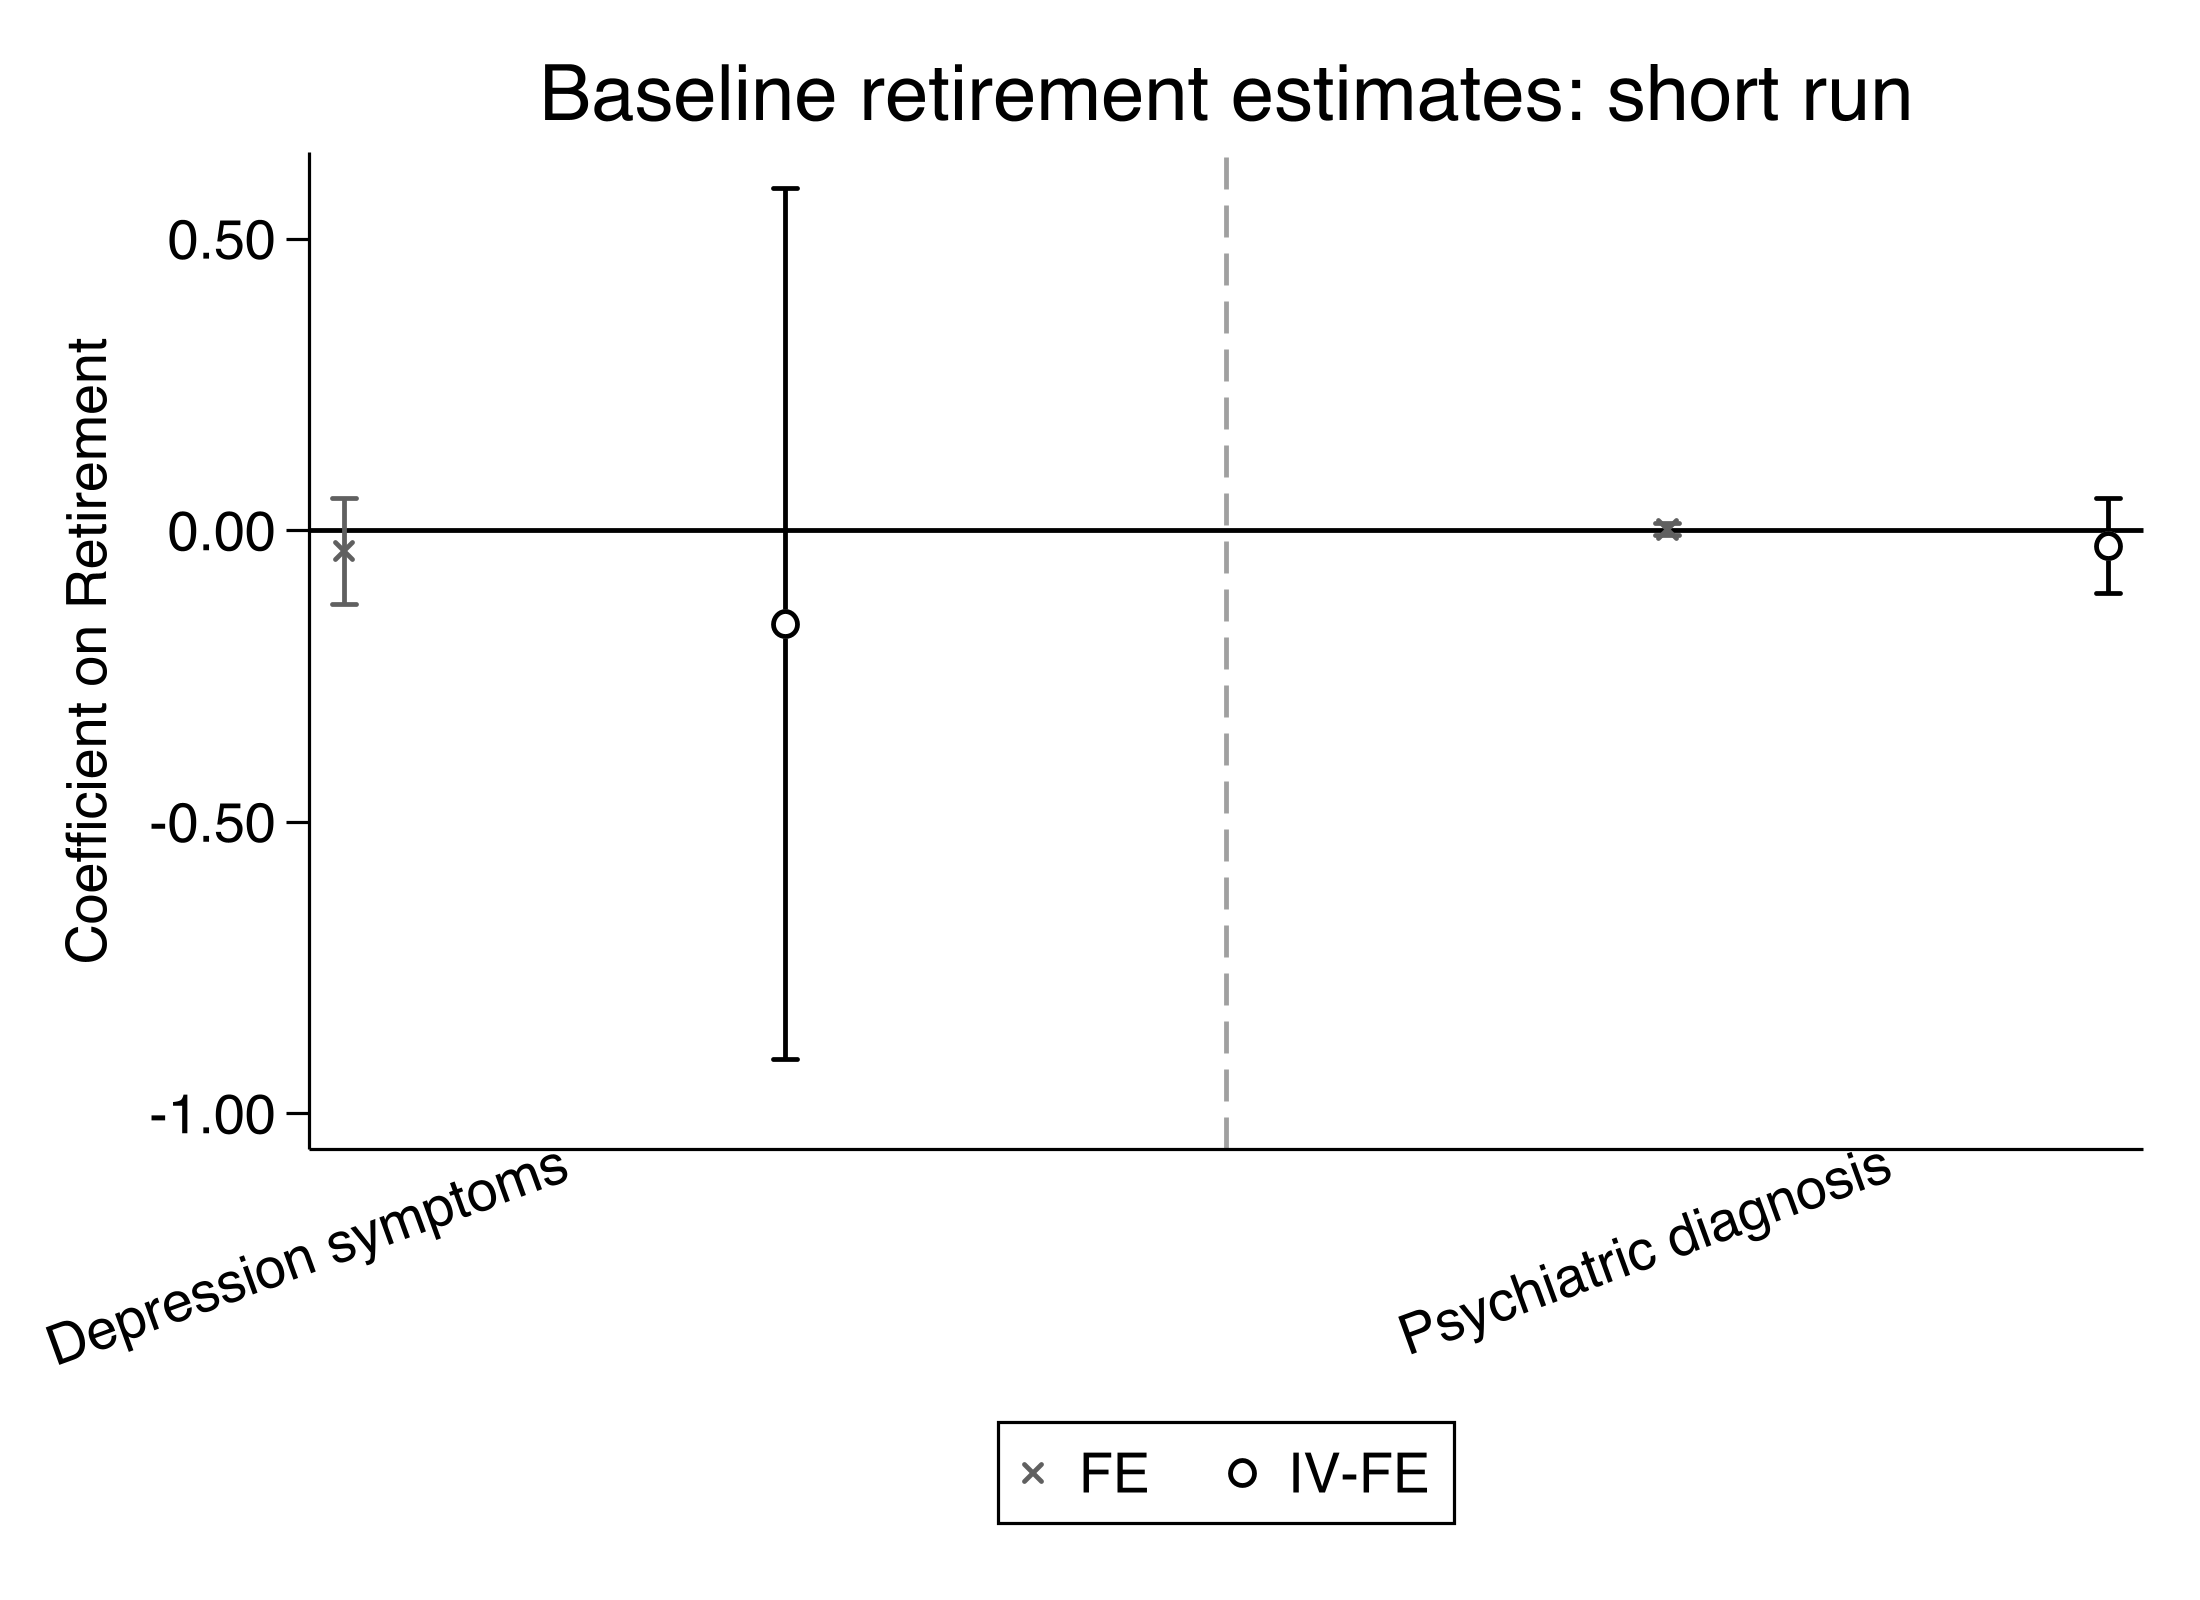
\includegraphics[width=0.9\textwidth]{Figure2.png}
\vspace*{-0.4cm}

\scriptsize{\singlespacing \emph{Notes:} Figure 2 plots the estimated effect of retirement on the two main mental health outcomes in the short-run sample (2009--2013). Red crosses report within-individual fixed effects (FE) estimates, while blue circles report instrumental-variables fixed-effects (IV-FE) estimates from Equation (1). Vertical bars denote 95\% confidence intervals. Depression is a binary indicator equal to one when the respondent reports four or more CES-D symptoms.}
\end{figure}

\begin{center}
[Table 2 around here]
\end{center}

Table 2 reports the short-run interacted IV estimates. The main all-sample result is mixed across the two mental health outcomes. In the short run, retiring in high-unemployment region-years is associated with a 5.1 percentage point decline in new psychiatric diagnoses, relative to a pre-retirement mean of 1.9\%. At the same time, the corresponding coefficient for the binary depression indicator is positive, about 7.8 percentage points, and marginally significant. This pattern suggests that any short-run relief from work-related stress is not broad enough to show up as lower depressive symptom prevalence. The subgroup estimates point to larger short-run declines in psychiatric diagnoses among men and white-collar workers, but the paper treats these heterogeneous estimates as secondary to the all-sample evidence. The minimum weak-identification statistics reported in the table are comfortably above conventional thresholds.

Table 3 turns to the longer-run period. The short-run decline in new psychiatric diagnoses disappears, while the crisis interaction becomes positive and statistically significant for the binary depression indicator in the full sample. The magnitude is economically meaningful: the coefficient of 0.082 implies an increase of roughly 97\% relative to the pre-retirement mean. This longer-run result is visible for both men and women and for both white-collar and blue-collar workers, although the subgroup estimates vary in precision. The longer-run evidence therefore points away from a durable mental health improvement from retiring in harder-hit labour markets.

\begin{center}
[Table 3 around here]
\end{center}

\subsection{Robustness checks} \label{sec:robustness}

Appendix B reports the diagnostic evidence for the baseline and interacted IV specifications. The statutory pension age remains a strong predictor of retirement, and the interaction instrument is also highly relevant in the crisis specification. Appendix C reports two additional checks. First, Table C1 shows that using the continuous CES-D symptom count yields the same qualitative longer-run pattern as the binary depression indicator: retirement in high-unemployment region-years is associated with worse depressive symptoms rather than better mental health. Second, Figures C1--C3 present event-study evidence for the binary depression indicator and new psychiatric diagnosis in the full sample and by sex. The event-study profiles are useful for visualising the timing of effects and do not suggest a clean and persistent improvement in broader depressive symptoms.

\section{Conclusion} \label{sec:discussion}

This paper studies whether retirement has different mental health consequences when it occurs in weak local labour markets. Using English panel data and an IV-FE design based on statutory pension-age eligibility, we find that the answer depends on which mental health outcome is examined and over what horizon. In the short run, retirement in high-unemployment region-years is associated with fewer new psychiatric diagnoses. But this short-run decline does not extend to the broader depression indicator, and it does not persist in the longer run.

The longer-run evidence is especially important. By 2009--2019, the interaction between retirement and crisis exposure is positive and statistically significant for the binary depression measure, while the earlier decline in psychiatric diagnoses has faded. The most credible interpretation is therefore not that retirement during a crisis uniformly improves mental health, but that short-run relief from work-related strain can coexist with, and eventually be outweighed by, a deterioration in broader depressive symptoms.

These findings help reconcile the mixed retirement--health literature. Retirement effects are shaped by macroeconomic conditions, and mental health outcomes that appear similar on the surface do not necessarily move together. For policy, the results suggest caution when viewing retirement as a straightforward buffer against downturns. Protecting mental health during and after labour-market shocks may require more than timely pension access; it may also require ongoing mental health support during the years that follow retirement.


\vspace{1.25cm}
\singlespacing
\section*{Conflict of interest statement}

The authors declare that they have no conflict of interest.

\section*{Data statement}

All databases are available under UK Data Services (UKDS) conditions.

\section*{Ethics statement}

No ethics approval was needed to perform this analysis. 


\newpage
\singlespacing
\setlength\bibsep{0pt}
\bibliographystyle{apalike}
\bibliography{bibliography.bib}



\clearpage



\section*{Tables} \label{sec:fig}
\addcontentsline{toc}{section}{Tables}
\clearpage

\begin{table}[h]
\centering
\caption{Descriptive statistics by employment status.}
\label{tab1}
\resizebox{0.9\textwidth}{!}{%
\begin{tabular}{@{}cccccc@{}}
\toprule
\multirow{2}{*}{\textbf{Variables}} & \multicolumn{2}{c}{\textbf{Employed}} & \multicolumn{2}{c}{\textbf{Retired}} & \multirow{2}{*}{\textbf{Test for Mean Differences}} \\
 & \textit{Mean} & \textit{SD} & \textit{Mean} & \textit{SD} &  \\ \cmidrule(r){1-6} 
\multicolumn{6}{l}{\textbf{Socio-demographics}} \\ \hline
\textit{Female} & 0.537 & 0.499 & 0.536 & 0.499 &  \\
\textit{Age} & 60.34 & 6.436 & 68.49 & 5.921 & *** \\
\textit{Married/Cohabiting} & 0.776 & 0.417 & 0.707 & 0.455 & *** \\
\textit{Household size} & 2.239 & 0.845 & 1.909 & 0.694 & *** \\
\textit{Home owner outright} & 0.590 & 0.492 & 0.819 & 0.385 & *** \\
\multicolumn{6}{l}{Education} \\
\textit{Never went or not yet finished} & 0.008 & 0.091 & 0.008 & 0.088 &  \\
\textit{Left school at 14 or below} & 0.015 & 0.122 & 0.029 & 0.167 & *** \\
\textit{O levels} & 0.459 & 0.498 & 0.471 & 0.499 &  \\
\textit{A levels} & 0.121 & 0.326 & 0.105 & 0.307 & *** \\
\textit{Higher education below degree} & 0.148 & 0.356 & 0.152 & 0.359 &  \\
\textit{Degree} & 0.248 & 0.432 & 0.235 & 0.424 & * \\\hline
\multicolumn{6}{l}{\textbf{Heterogeneity variables}} \\\hline
\textit{Blue-collar worker} & 0.482 & 0.500 & 0.507 & 0.500 & *** \\
\textit{High-unemployment region-year} & 0.263 & 0.440 & 0.295 & 0.456 & *** \\
\textit{Above state pension age} & 0.366 & 0.482 & 0.893 & 0.309 & *** \\
\textit{Top financial wealth quartile} & 0.230 & 0.421 & 0.276 & 0.447 & *** \\\hline
\multicolumn{6}{l}{\textbf{Regional Characteristics}} \\\hline
\multicolumn{6}{l}{Population Density for Postcode Sectors} \\
\textit{First quintile (least dense)} & 0.201 & 0.401 & 0.202 & 0.401 &  \\
\textit{Second quintile} & 0.245 & 0.430 & 0.253 & 0.435 &  \\
\textit{Third quintile} & 0.219 & 0.414 & 0.238 & 0.426 & *** \\
\textit{Fourth quintile} & 0.190 & 0.393 & 0.184 & 0.387 &  \\
\textit{Fifth quintile (most dense)} & 0.144 & 0.351 & 0.123 & 0.329 & *** \\
\multicolumn{6}{l}{Index of Multiple Deprivation Score} \\
\textit{First quintile (least deprived)} & 0.278 & 0.448 & 0.286 & 0.452 &  \\
\textit{Second quintile} & 0.268 & 0.443 & 0.267 & 0.442 &  \\
\textit{Third quintile} & 0.206 & 0.405 & 0.199 & 0.400 &  \\
\textit{Fourth quintile} & 0.149 & 0.356 & 0.162 & 0.368 & ** \\
\textit{Fifth quintile (most deprived)} & 0.098 & 0.298 & 0.087 & 0.281 & ** \\\hline
\multicolumn{6}{l}{\textit{\textbf{Pension characteristics and financial variables}}} \\\hline
\textit{Member of private pension scheme} & 0.800 & 0.400 & 0.792 & 0.406 &  \\
\textit{State pension income (£ per week)} & 64.99 & 90.45 & 176.93 & 97.20 & *** \\
\textit{Under financial strain} & 0.044 & 0.204 & 0.028 & 0.165 & *** \\\hline
\multicolumn{6}{l}{\textit{\textbf{Health related-behaviours}}} \\\hline
\textit{Never smoked} & 0.380 & 0.485 & 0.362 & 0.481 & ** \\
\textit{Vigorous physical activity at least weekly} & 0.393 & 0.488 & 0.349 & 0.477 & *** \\
\textit{Private health insurance} & 0.197 & 0.398 & 0.100 & 0.300 & *** \\\hline
\multicolumn{1}{l}{Observations} & \multicolumn{2}{c}{8,900} & \multicolumn{2}{c}{6,588} &  \\ \bottomrule \bottomrule
\end{tabular}%

 }

\tiny{{\singlespacing \emph{Notes:} Significance levels: ***p$\prec$0.01; **p$\prec$0.05; *p$\prec$0.1. The table reports sample means and standard deviations for employed and retired observations. The last column reports t-tests for equality of means. Variables shown correspond to the main regression controls and the heterogeneity variables used in the paper.}}
 
\end{table}

\newpage
\begin{table}[!ht]
\centering
\renewcommand{\arraystretch}{0.9}
\caption{Retirement in high-unemployment region-years and mental health: short-run estimates (2009--2013)}
\label{tab2}
\resizebox{\textwidth}{!}{%
\begin{tabular}{@{}lccccc@{}}
\toprule
 & \textbf{All sample} & \textbf{Men} & \textbf{Women} & \textbf{White-collar} & \textbf{Blue-collar} \\ \midrule
\multicolumn{6}{l}{\textbf{Panel A. Depression symptoms (CES-D $\geq$ 4)}} \\
Retired $\times$ high unemployment & \begin{tabular}[c]{@{}c@{}}0.078*\\ (0.042)\end{tabular} & \begin{tabular}[c]{@{}c@{}}0.001\\ (0.051)\end{tabular} & \begin{tabular}[c]{@{}c@{}}0.102\\ (0.063)\end{tabular} & \begin{tabular}[c]{@{}c@{}}0.097\\ (0.065)\end{tabular} & \begin{tabular}[c]{@{}c@{}}0.039\\ (0.060)\end{tabular} \\
Pre-retirement mean & 0.089 & 0.067 & 0.108 & 0.078 & 0.101 \\
Effect size (\%) & 87.5 & 1.5 & 93.8 & 124.6 & 39.2 \\
Min. weak-ID F-statistic & 54.24 & 32.89 & 29.68 & 17.29 & 39.08 \\
$R^2$ & 0.010 & 0.020 & 0.004 & -0.115 & 0.005 \\
Observations & 9,951 & 4,650 & 5,301 & 5,028 & 4,718 \\ \midrule
\multicolumn{6}{l}{\textbf{Panel B. New psychiatric diagnosis}} \\
Retired $\times$ high unemployment & \begin{tabular}[c]{@{}c@{}}-0.051**\\ (0.023)\end{tabular} & \begin{tabular}[c]{@{}c@{}}-0.052*\\ (0.029)\end{tabular} & \begin{tabular}[c]{@{}c@{}}-0.044\\ (0.035)\end{tabular} & \begin{tabular}[c]{@{}c@{}}-0.066*\\ (0.038)\end{tabular} & \begin{tabular}[c]{@{}c@{}}-0.031\\ (0.029)\end{tabular} \\
Pre-retirement mean & 0.019 & 0.015 & 0.023 & 0.019 & 0.020 \\
Effect size (\%) & -265.5 & -344.7 & -190.0 & -348.1 & -158.0 \\
Min. weak-ID F-statistic & 54.24 & 32.89 & 29.68 & 17.29 & 39.08 \\
$R^2$ & -0.002 & 0.004 & -0.008 & 0.000 & 0.011 \\
Observations & 9,951 & 4,650 & 5,301 & 5,028 & 4,718 \\ \bottomrule
\end{tabular}%
}
\tiny{{\singlespacing \emph{Notes:} IV-FE estimates from Equation (2). The reported coefficient is the interaction between retirement and the high-unemployment indicator. Depression is a binary indicator equal to one when the respondent reports four or more CES-D symptoms. All specifications include individual fixed effects, wave indicators, and the full set of controls described in Section 4. Clustered standard errors at the individual level are in parentheses. Significance levels: ***p$\prec$0.01; **p$\prec$0.05; *p$\prec$0.1.}}
\end{table}

\newpage
\begin{table}[!ht]
\centering
\renewcommand{\arraystretch}{0.9}
\caption{Retirement in high-unemployment region-years and mental health: longer-run estimates (2009--2019)}
\label{tab3}
\resizebox{\textwidth}{!}{%
\begin{tabular}{@{}lccccc@{}}
\toprule
 & \textbf{All sample} & \textbf{Men} & \textbf{Women} & \textbf{White-collar} & \textbf{Blue-collar} \\ \midrule
\multicolumn{6}{l}{\textbf{Panel A. Depression symptoms (CES-D $\geq$ 4)}} \\
Retired $\times$ high unemployment & \begin{tabular}[c]{@{}c@{}}0.082***\\ (0.023)\end{tabular} & \begin{tabular}[c]{@{}c@{}}0.066**\\ (0.029)\end{tabular} & \begin{tabular}[c]{@{}c@{}}0.087**\\ (0.037)\end{tabular} & \begin{tabular}[c]{@{}c@{}}0.076**\\ (0.032)\end{tabular} & \begin{tabular}[c]{@{}c@{}}0.078**\\ (0.035)\end{tabular} \\
Pre-retirement mean & 0.084 & 0.063 & 0.103 & 0.073 & 0.097 \\
Effect size (\%) & 97.2 & 104.2 & 84.5 & 104.2 & 80.4 \\
Min. weak-ID F-statistic & 97.56 & 52.26 & 57.03 & 37.74 & 66.28 \\
$R^2$ & 0.005 & 0.008 & 0.003 & -0.004 & 0.008 \\
Observations & 14,774 & 6,857 & 7,917 & 7,520 & 7,097 \\ \midrule
\multicolumn{6}{l}{\textbf{Panel B. New psychiatric diagnosis}} \\
Retired $\times$ high unemployment & \begin{tabular}[c]{@{}c@{}}-0.013\\ (0.013)\end{tabular} & \begin{tabular}[c]{@{}c@{}}-0.021\\ (0.016)\end{tabular} & \begin{tabular}[c]{@{}c@{}}-0.001\\ (0.020)\end{tabular} & \begin{tabular}[c]{@{}c@{}}-0.011\\ (0.020)\end{tabular} & \begin{tabular}[c]{@{}c@{}}-0.013\\ (0.017)\end{tabular} \\
Pre-retirement mean & 0.017 & 0.014 & 0.020 & 0.017 & 0.017 \\
Effect size (\%) & -73.7 & -147.9 & -3.5 & -63.5 & -74.0 \\
Min. weak-ID F-statistic & 97.56 & 52.26 & 57.03 & 37.74 & 66.28 \\
$R^2$ & -0.010 & 0.003 & -0.015 & -0.034 & 0.007 \\
Observations & 14,774 & 6,857 & 7,917 & 7,520 & 7,097 \\ \bottomrule
\end{tabular}%
}
\tiny{{\singlespacing \emph{Notes:} IV-FE estimates from Equation (2) using the longer-run sample. The reported coefficient is the interaction between retirement and the high-unemployment indicator. Depression is a binary indicator equal to one when the respondent reports four or more CES-D symptoms. All specifications include individual fixed effects, wave indicators, and the full set of controls described in Section 4. Clustered standard errors at the individual level are in parentheses. Significance levels: ***p$\prec$0.01; **p$\prec$0.05; *p$\prec$0.1.}}
\end{table}


\clearpage
%\appendix
\section*{Appendix A. English Longitudinal Study of Ageing (ELSA)} 
\label{sec:appendixa}
\setcounter{table}{0}
\renewcommand{\thetable}{A\arabic{table}}
\addcontentsline{toc}{section}{Appendix A}
\singlespacing
\small
The English Longitudinal Study of Ageing (ELSA) began in 2002 as a large-scale longitudinal panel study focusing on individuals aged 50 and over, along with their partners, who live in private households in England. The original sample was drawn from households that had previously participated in the Health Survey for England (HSE) between 1998 and 2001. Participants are interviewed every two years, allowing researchers to observe changes over time, track the progression of aging, and investigate cause-and-effect relationships. ELSA is part of a network of aging studies worldwide, which includes the Health and Retirement Study (HRS) in the United States and the Survey of Health, Ageing, and Retirement in Europe (SHARE), thus facilitating international research on aging.

\begin{table}[htb!]
\centering
\caption{Fieldwork periods by wave}
\label{tabA1}
\resizebox{0.35\textwidth}{!}{%
\begin{tabular}{@{}cc@{}}
\toprule
\multicolumn{2}{c}{\textbf{Fieldwork period}} \\ \midrule
\textbf{Wave 1} & March 2002 – March 2003 \\
\textbf{Wave 2} & June 2004 – July 2005 \\
\textbf{Wave 3} & May 2006 – August 2007 \\
\textbf{Wave 4} & May 2008 – July 2009 \\
\textbf{Wave 5} & June 2010 – July 2011 \\
\textbf{Wave 6} & May 2012 – June 2013 \\
\textbf{Wave 7} & June 2014 – May 2015 \\
\textbf{Wave 8} & May 2016 – June 2017 \\
\textbf{Wave 9} & June 2018 – July 2019 \\ \bottomrule
\end{tabular}%
}
\end{table}


Table A2 summarises the number of productive interviews archived at each wave, along with the counts of Core Member and Partner interviews. It also provides a detailed analysis of response rates, including field contact rates, overall response rates, and cohort response rates for each ELSA wave.

\begin{table}[htb!]
\centering
\caption{Number of interviews by waves}
\label{tabA2}
\resizebox{0.6\textwidth}{!}{%
\begin{tabular}{@{}ccc@{}}
\hline
\textbf{} & \textbf{Total archived interviews} & \textbf{Core Member interviews} \\ \hline
\textbf{Wave 1} & 12,099 & 11,391 \\
\textbf{Wave 2} & 9,432 & 8,780 \\
\textbf{Wave 3} & 9,771 & 8,810 \\
\textbf{Wave 4} & 11,050 & 9,886 \\
\textbf{Wave 5} & 10,274 & 9,090 \\
\textbf{Wave 6} & 10,601 & 9,169 \\
\textbf{Wave 7} & 9,666 & 8,249 \\
\textbf{Wave 8} & 8,445 & 7,223 \\
\textbf{Wave 9} & 8,736 & 7,289 \\ \hline
\end{tabular}%
}
\end{table}


\newpage
In our analysis, we selected a subsample of active individuals who defined their employment status as employee, self-employed, temporarily sick or disabled, or seeking work. They also need not have any kind of chronic condition—please refer to Table A3. We then follow this subsample across time and record them when they retire from working. Table A3 shows the number of observations and individuals available in the dataset.

\begin{table}[htb!]

\centering
\caption{Observations and individual panel across waves}
\begin{adjustwidth}{-2cm}{}
\label{tabA3}
\resizebox{1.15\textwidth}{!}{%
\begin{tabular}{@{}cccccccccc@{}}
\toprule
 & \textbf{\begin{tabular}[c]{@{}c@{}}2002/03\\ Wave 1\end{tabular}} & \textbf{\begin{tabular}[c]{@{}c@{}}2004/05 \\ Wave 2\end{tabular}} & \textbf{\begin{tabular}[c]{@{}c@{}}2006/07 \\ Wave 3\end{tabular}} & \textbf{\begin{tabular}[c]{@{}c@{}}2008/09\\ Wave 4\end{tabular}} & \textbf{\begin{tabular}[c]{@{}c@{}}2010/11 \\ Wave 5\end{tabular}} & \textbf{\begin{tabular}[c]{@{}c@{}}2012/13 \\ Wave 6\end{tabular}} & \textbf{\begin{tabular}[c]{@{}c@{}}2014/15\\  Wave 7\end{tabular}} & \textbf{\begin{tabular}[c]{@{}c@{}}2016/17 \\ Wave 8\end{tabular}} & \textbf{\begin{tabular}[c]{@{}c@{}}2018/19 \\ Wave 9\end{tabular}} \\ \midrule
\textit{Working} & 2,668 & 2,185 & 1,752 & 1,402 & 1,173 & 898 & 661 & 483 & 346 \\
\textit{Retirement} & 0 & 278 & 444 & 622 & 827 & 1,012 & 1,109 & 1,146 & 1,150 \\
\textit{Total Obs.} & 2,668 & 2,463 & 2,196 & 2,024 & 2,000 & 1,910 & 1,770 & 1,629 & 1,496 \\
\textit{Num IDs} & 547 & 499 & 374 & 304 & 215 & 203 & 188 & 186 & 152 \\ \bottomrule
\end{tabular}%
}
\end{adjustwidth}
\end{table}


We have an unbalanced panel dataset of individuals, with approximately 76\% of them answering the questionnaire across all the waves included in the short-term analysis. This figure increases to around 87\% when we include those who missed recording their answers in just one of the five subsequent waves, indicating a successful follow-up.

\begin{table}[h]
\begin{adjustwidth}{-1.75cm}{}
\centering
\caption{Unbalanced panel observation (short-term analysis (2004-2013)}
\label{tabA4}
\resizebox{\textwidth}{!}{%
\begin{tabular}{cccccccc}
\hline
$Wave_{t}$ & \textbf{$Wave_{t+1}$} & \textbf{$Wave_{t+2}$} & \textbf{$Wave_{t+3}$} & \textbf{$Wave_{t+4}$} & \textbf{$Wave_{t+5}$} & \textbf{Observations} & \textbf{Percent} \\ \hline
\textit{\checkmark} & \textit{\checkmark} &  &  &  &  & 308 & 2.91 \\
\textit{\checkmark} & \textit{\checkmark} & \textit{\checkmark} &  &  &  & 548 & 5.17 \\
\textit{\checkmark} & \textit{\checkmark} & \textit{\checkmark} & \textit{\checkmark} &  &  & 555 & 5.24 \\
\textit{\checkmark} & \textit{\checkmark} & \textit{\checkmark} & \textit{\checkmark} & \textit{\checkmark} &  & 1,132 & 10.69 \\
\textit{\checkmark} & \textit{\checkmark} & \textit{\checkmark} & \textit{\checkmark} & \textit{\checkmark} & \textit{\checkmark} & 8,050 & 75.99 \\  \hline 
\end{tabular}%
}
\end{adjustwidth}
\end{table}

\newpage
Table A5 presents the results of two informal tests examining the severity of selective attrition. We first expand the rows in the dataset to create a nominally balanced format so that each identifier includes the same list of time periods, filling in waves without data with missing values. We then define a complete-cases selection indicator. The first specification uses new psychiatric diagnosis as the dependent variable, while the second uses attrition itself as the dependent variable, controlling for the main specification variables.


\begin{table}[h]
\centering

\renewcommand{\arraystretch}{0.7}
\caption{Attrition tests}
\begin{adjustwidth}{-1.25cm}{}
\label{tab5}
\resizebox{\textwidth}{!}{%
\begin{tabular}{@{}ccccccc@{}}
\toprule
 & \multicolumn{3}{c}{\textbf{\begin{tabular}[c]{@{}c@{}}PANEL A\\ Dependent variable: New \\ psychiatric diagnosis\end{tabular}}} & \multicolumn{3}{c}{\textbf{\begin{tabular}[c]{@{}c@{}}PANEL B\\ Dependent variable: Attrite\end{tabular}}} \\ \midrule
 & \textit{All} & \textit{Men} & \textit{Women} & \textit{All} & \textit{Men} & \textit{Women} \\ \hline
Attrite & \begin{tabular}[c]{@{}c@{}}0.002\\ (0.004)\end{tabular} & \begin{tabular}[c]{@{}c@{}}0.005\\ (0.005)\end{tabular} & \begin{tabular}[c]{@{}c@{}}-0.000\\ (0.006)\end{tabular} &  &  &  \\
Attrite x Retirement & \begin{tabular}[c]{@{}c@{}}0.007\\ (0.008)\end{tabular} & \begin{tabular}[c]{@{}c@{}}0.001\\ (0.010)\end{tabular} & \begin{tabular}[c]{@{}c@{}}0.015\\ (0.013)\end{tabular} &  &  &  \\
\begin{tabular}[c]{@{}c@{}}New psychiatric \\ diagnosis\end{tabular} &  &  &  & \begin{tabular}[c]{@{}c@{}}-0.002 \\ (0.014)\end{tabular} & \begin{tabular}[c]{@{}c@{}}0.007 \\ (0.021)\end{tabular} & \begin{tabular}[c]{@{}c@{}}-0.010\\ (0.018)\end{tabular} \\
Control variables & Yes & Yes & Yes & Yes & Yes & Yes \\
Observations & 10,273 & 4,793 & 5,480 & 10,273 & 4,793 & 5,480 \\
IDs & 2,638 & 1,229 & 1,409 & 2,638 & 1,229 & 1,409 \\ \bottomrule
\end{tabular}%
}
\end{adjustwidth}
\end{table}

\newpage
\section*{Appendix B. Instrument validity diagnostics} \label{sec:appendixB}
\setcounter{table}{0}
\renewcommand{\thetable}{B\arabic{table}}
\addcontentsline{toc}{section}{Appendix B}

\begin{table}[h]
\centering
\caption{Baseline IV diagnostics for the short-run sample (2009--2013)}
\label{tabB1}
\resizebox{0.92\textwidth}{!}{%
\begin{tabular}{@{}lcccc@{}}
\toprule
 & \textbf{All sample} & \textbf{Women} & \textbf{Blue-collar} & \textbf{High-unemployment} \\ \midrule
\multicolumn{5}{l}{\textbf{Panel A. Depression symptoms (CES-D $\geq$ 4)}} \\
Kleibergen-Paap LM statistic & 102.71 & 52.58 & 77.83 & 36.30 \\
Weak-ID F-statistic & 104.31 & 53.40 & 80.25 & 36.39 \\
Observations & 9,951 & 5,301 & 4,718 & 6,235 \\ \midrule
\multicolumn{5}{l}{\textbf{Panel B. New psychiatric diagnosis}} \\
Kleibergen-Paap LM statistic & 102.71 & 52.58 & 77.83 & 36.30 \\
Weak-ID F-statistic & 104.31 & 53.40 & 80.25 & 36.39 \\
Observations & 9,951 & 5,301 & 4,718 & 6,235 \\ \bottomrule
\end{tabular}%
}
\tiny{{\singlespacing \emph{Notes:} Appendix Table B1 reports the baseline IV diagnostic statistics for the two mental-health outcomes in the short-run sample. The instrument is statutory pension-age eligibility.}}
\end{table}

\newpage
\begin{table}[h]
\centering
\caption{Interacted IV diagnostics for the short-run crisis specification (2009--2013)}
\label{tabB2}
\resizebox{\textwidth}{!}{%
\begin{tabular}{@{}lccccc@{}}
\toprule
 & \textbf{All sample} & \textbf{Men} & \textbf{Women} & \textbf{White-collar} & \textbf{Blue-collar} \\ \midrule
\multicolumn{6}{l}{\textbf{Panel A. Depression symptoms (CES-D $\geq$ 4)}} \\
Kleibergen-Paap LM statistic & 105.19 & 51.71 & 53.10 & 27.19 & 82.93 \\
Weak-ID F-statistic & 53.21 & 25.76 & 26.72 & 13.59 & 42.66 \\
Observations & 9,951 & 4,650 & 5,301 & 5,028 & 4,718 \\ \midrule
\multicolumn{6}{l}{\textbf{Panel B. New psychiatric diagnosis}} \\
Kleibergen-Paap LM statistic & 105.19 & 51.71 & 53.10 & 27.19 & 82.93 \\
Weak-ID F-statistic & 53.21 & 25.76 & 26.72 & 13.59 & 42.66 \\
Observations & 9,951 & 4,650 & 5,301 & 5,028 & 4,718 \\ \bottomrule
\end{tabular}%
}
\tiny{{\singlespacing \emph{Notes:} Appendix Table B2 reports diagnostic statistics for the interacted IV specification in Equation (2), where retirement and retirement $\times$ high unemployment are instrumented with pension-age eligibility and its interaction with high unemployment.}}
\end{table}

\newpage
\section*{Appendix C. Alternative depression measure and event-study evidence} \label{sec:appendixC}
\setcounter{table}{0}
\renewcommand{\thetable}{C\arabic{table}}
\setcounter{figure}{0}
\renewcommand{\thefigure}{C\arabic{figure}}
\addcontentsline{toc}{section}{Appendix C}

Appendix C presents two supporting pieces of evidence. First, Table C1 re-estimates the crisis specification using the continuous CES-D symptom count, which ranges from 0 to 8. Second, Figures C1--C3 report event-study estimates for the two main mental-health outcomes in the full sample and separately by sex.

\begin{table}[h]
\centering
\caption{Continuous CES-D symptom count as an alternative depression measure}
\label{tabC1}
\resizebox{0.82\textwidth}{!}{%
\begin{tabular}{@{}lcc@{}}
\toprule
 & \textbf{Short run (2009--2013)} & \textbf{Longer run (2009--2019)} \\ \midrule
Retired $\times$ high unemployment & \begin{tabular}[c]{@{}c@{}}0.266\\ (0.214)\end{tabular} & \begin{tabular}[c]{@{}c@{}}0.342***\\ (0.122)\end{tabular} \\
Pre-retirement mean & 1.049 & 1.020 \\
Effect size (\%) & 25.3 & 33.5 \\
Min. weak-ID F-statistic & 54.24 & 97.56 \\
$R^2$ & 0.021 & 0.009 \\
Observations & 9,951 & 14,774 \\ \bottomrule
\end{tabular}%
}
\tiny{{\singlespacing \emph{Notes:} IV-FE estimates from Equation (2) using the continuous CES-D symptom count instead of the binary depression indicator. Clustered standard errors at the individual level are in parentheses. Significance levels: ***p$\prec$0.01; **p$\prec$0.05; *p$\prec$0.1.}}
\end{table}

\newpage
\begin{figure}[htb!]
\caption{Event-study estimates in the full sample}
\label{figC1}
\begin{center}
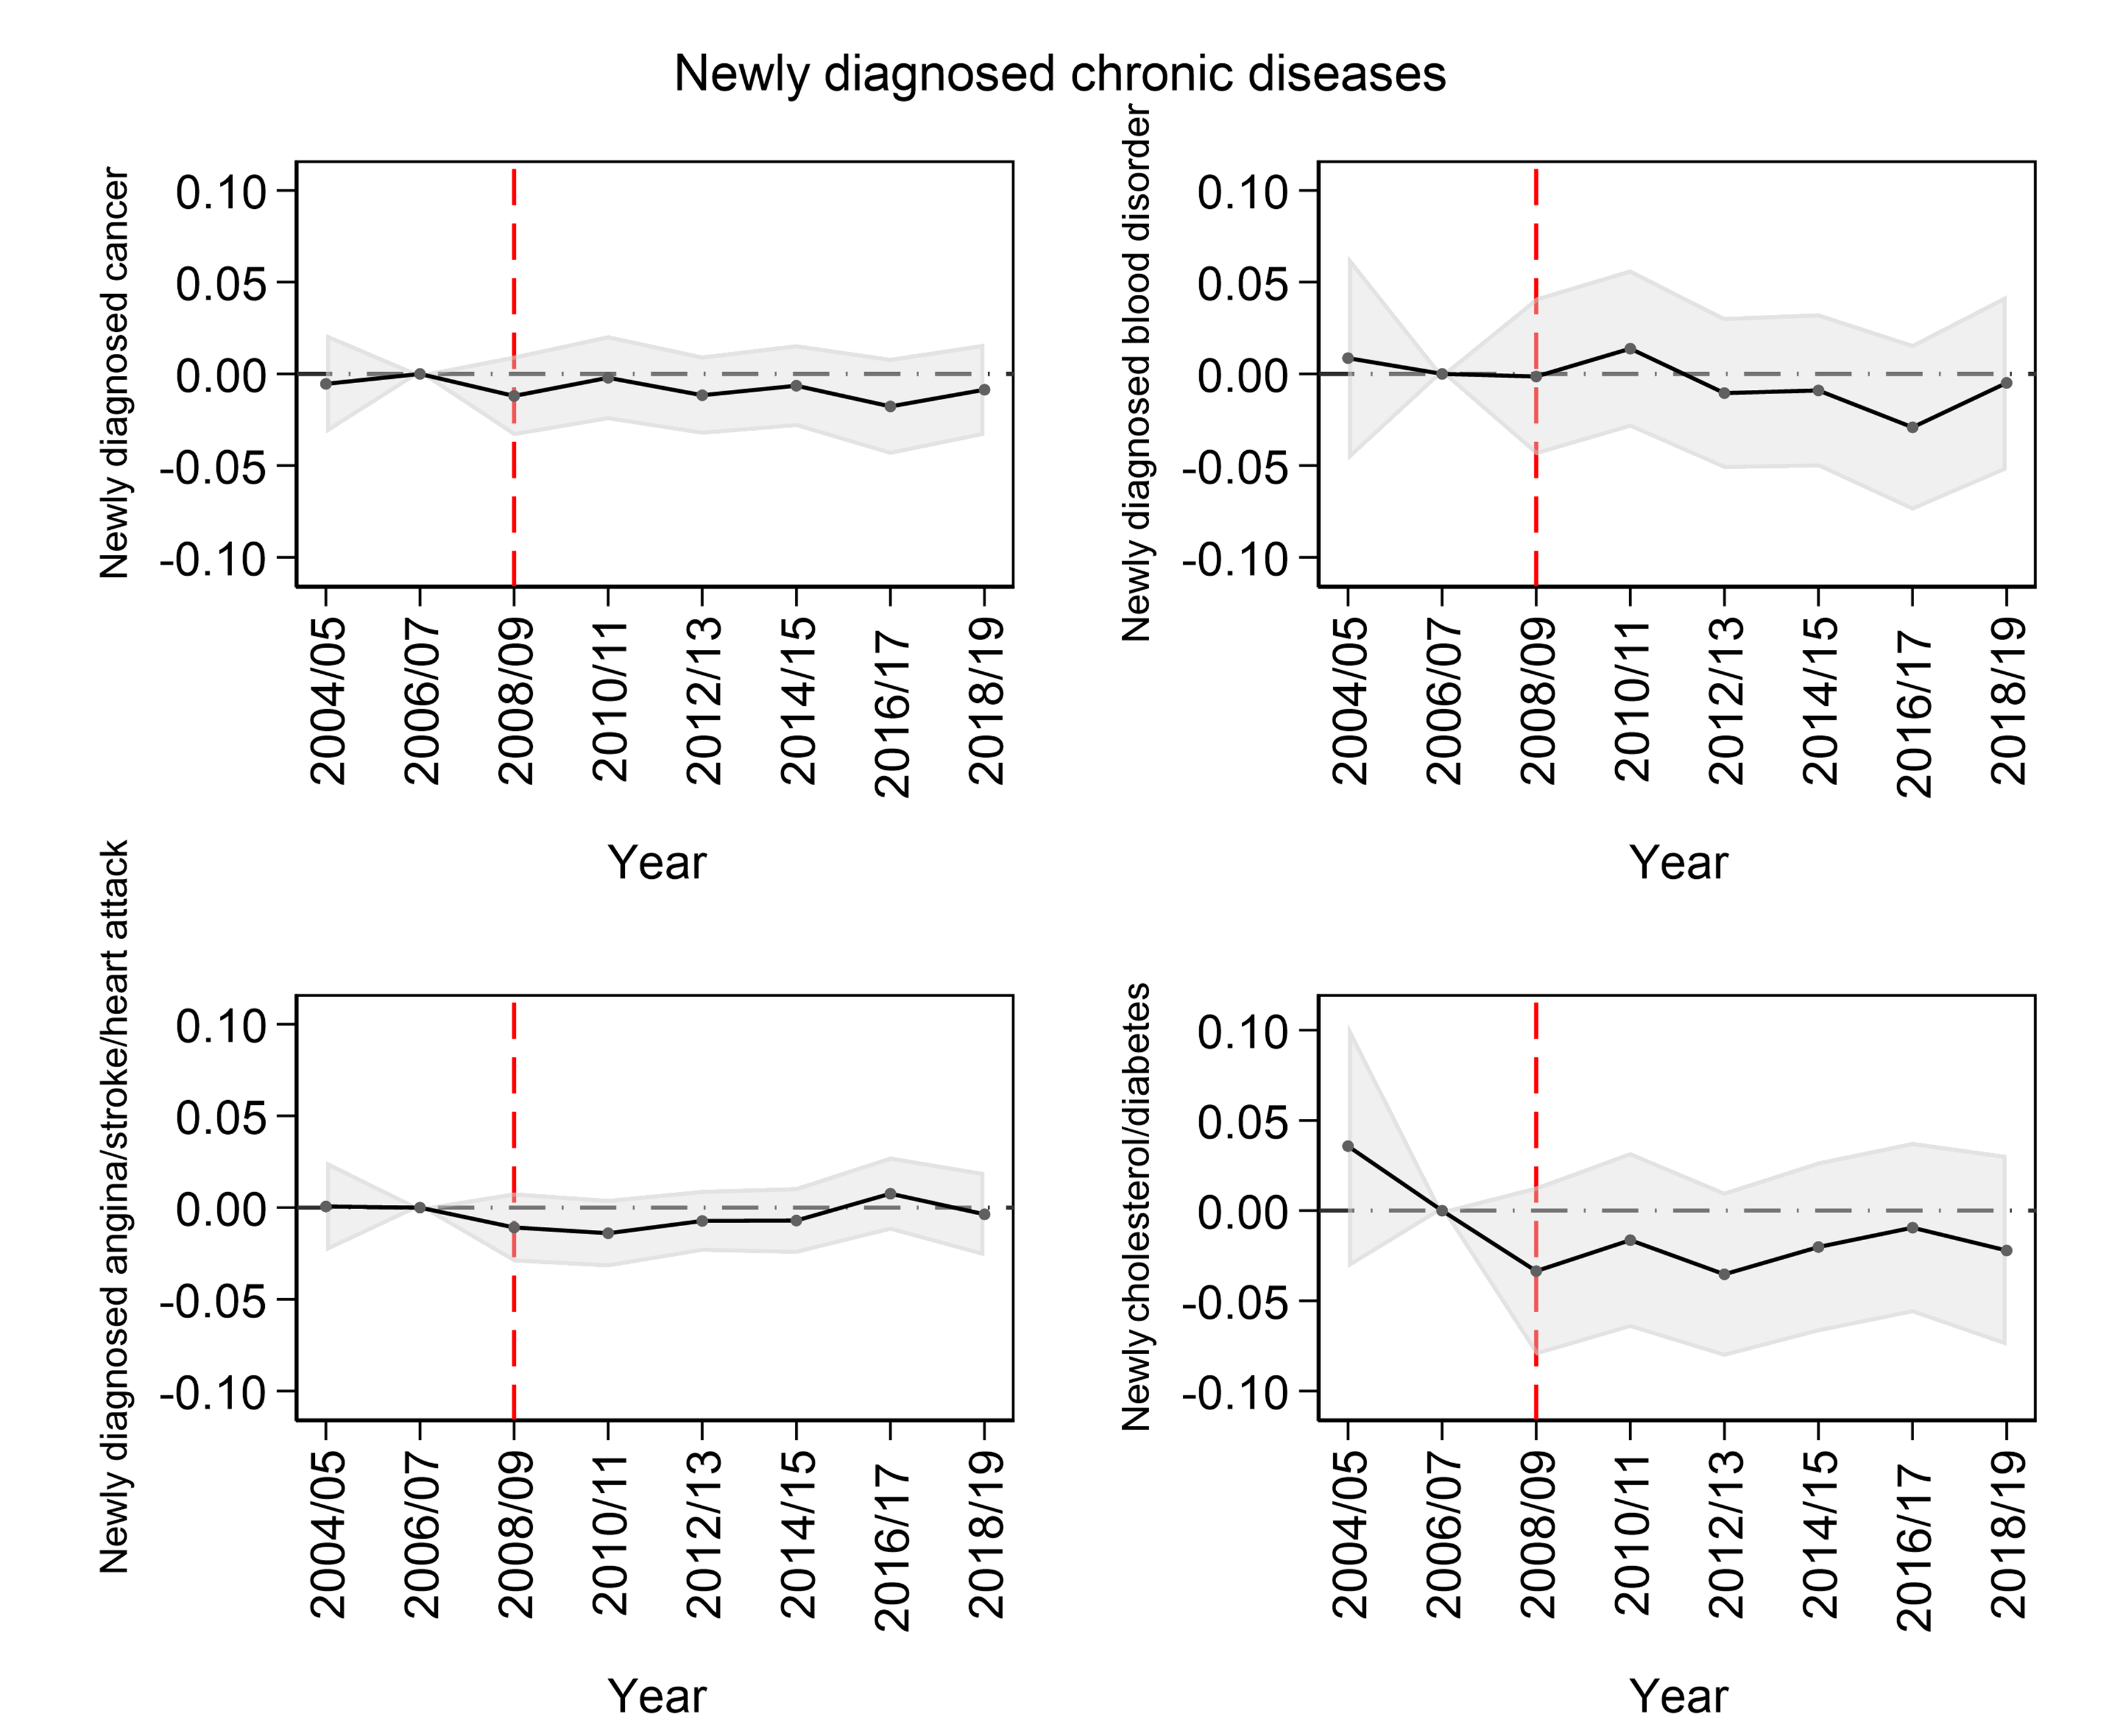
\includegraphics[width=0.72\textwidth]{eventstudy1.png}
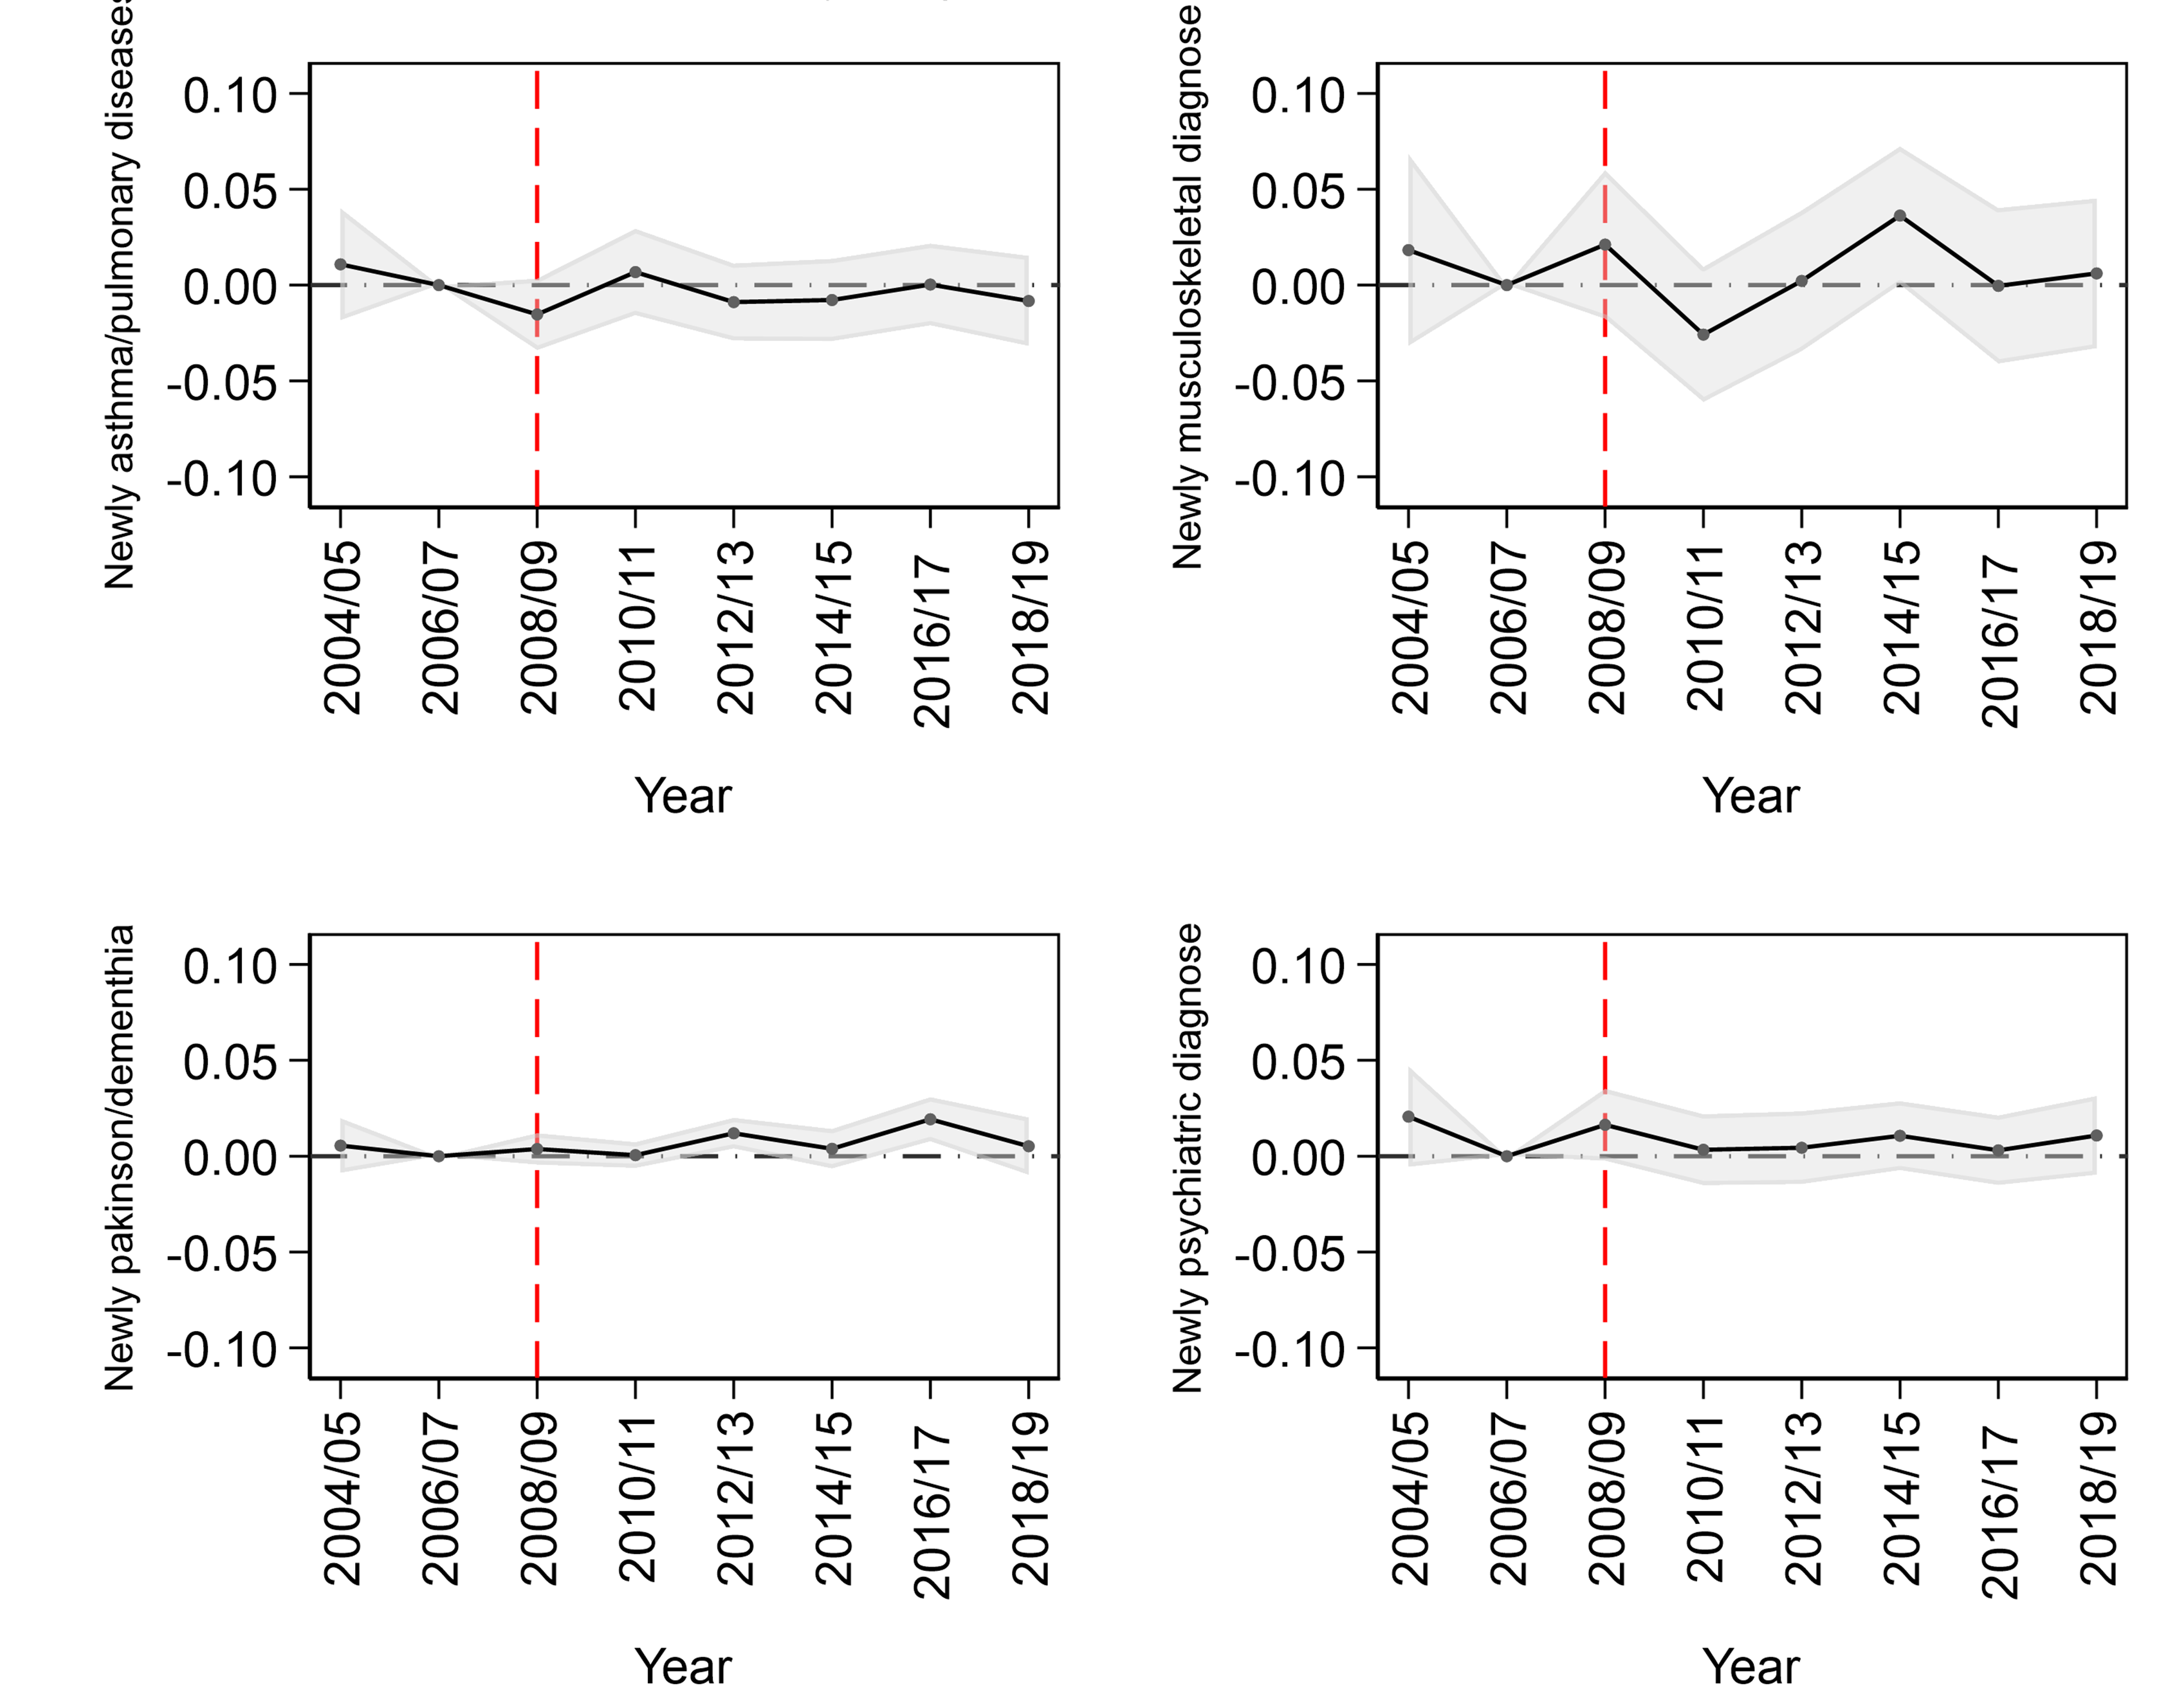
\includegraphics[width=0.72\textwidth]{eventstudy1.2.png}
\end{center}
\scriptsize{\singlespacing \emph{Notes:} The top panel reports event-study estimates for depression symptoms, defined as CES-D $\geq$ 4, and the bottom panel reports event-study estimates for new psychiatric diagnosis. Both figures are estimated on the full sample with individual fixed effects, wave effects, and the standard control set.}
\end{figure}

\newpage
\begin{figure}[htb!]
\caption{Event-study estimates for men}
\label{figC2}
\centering
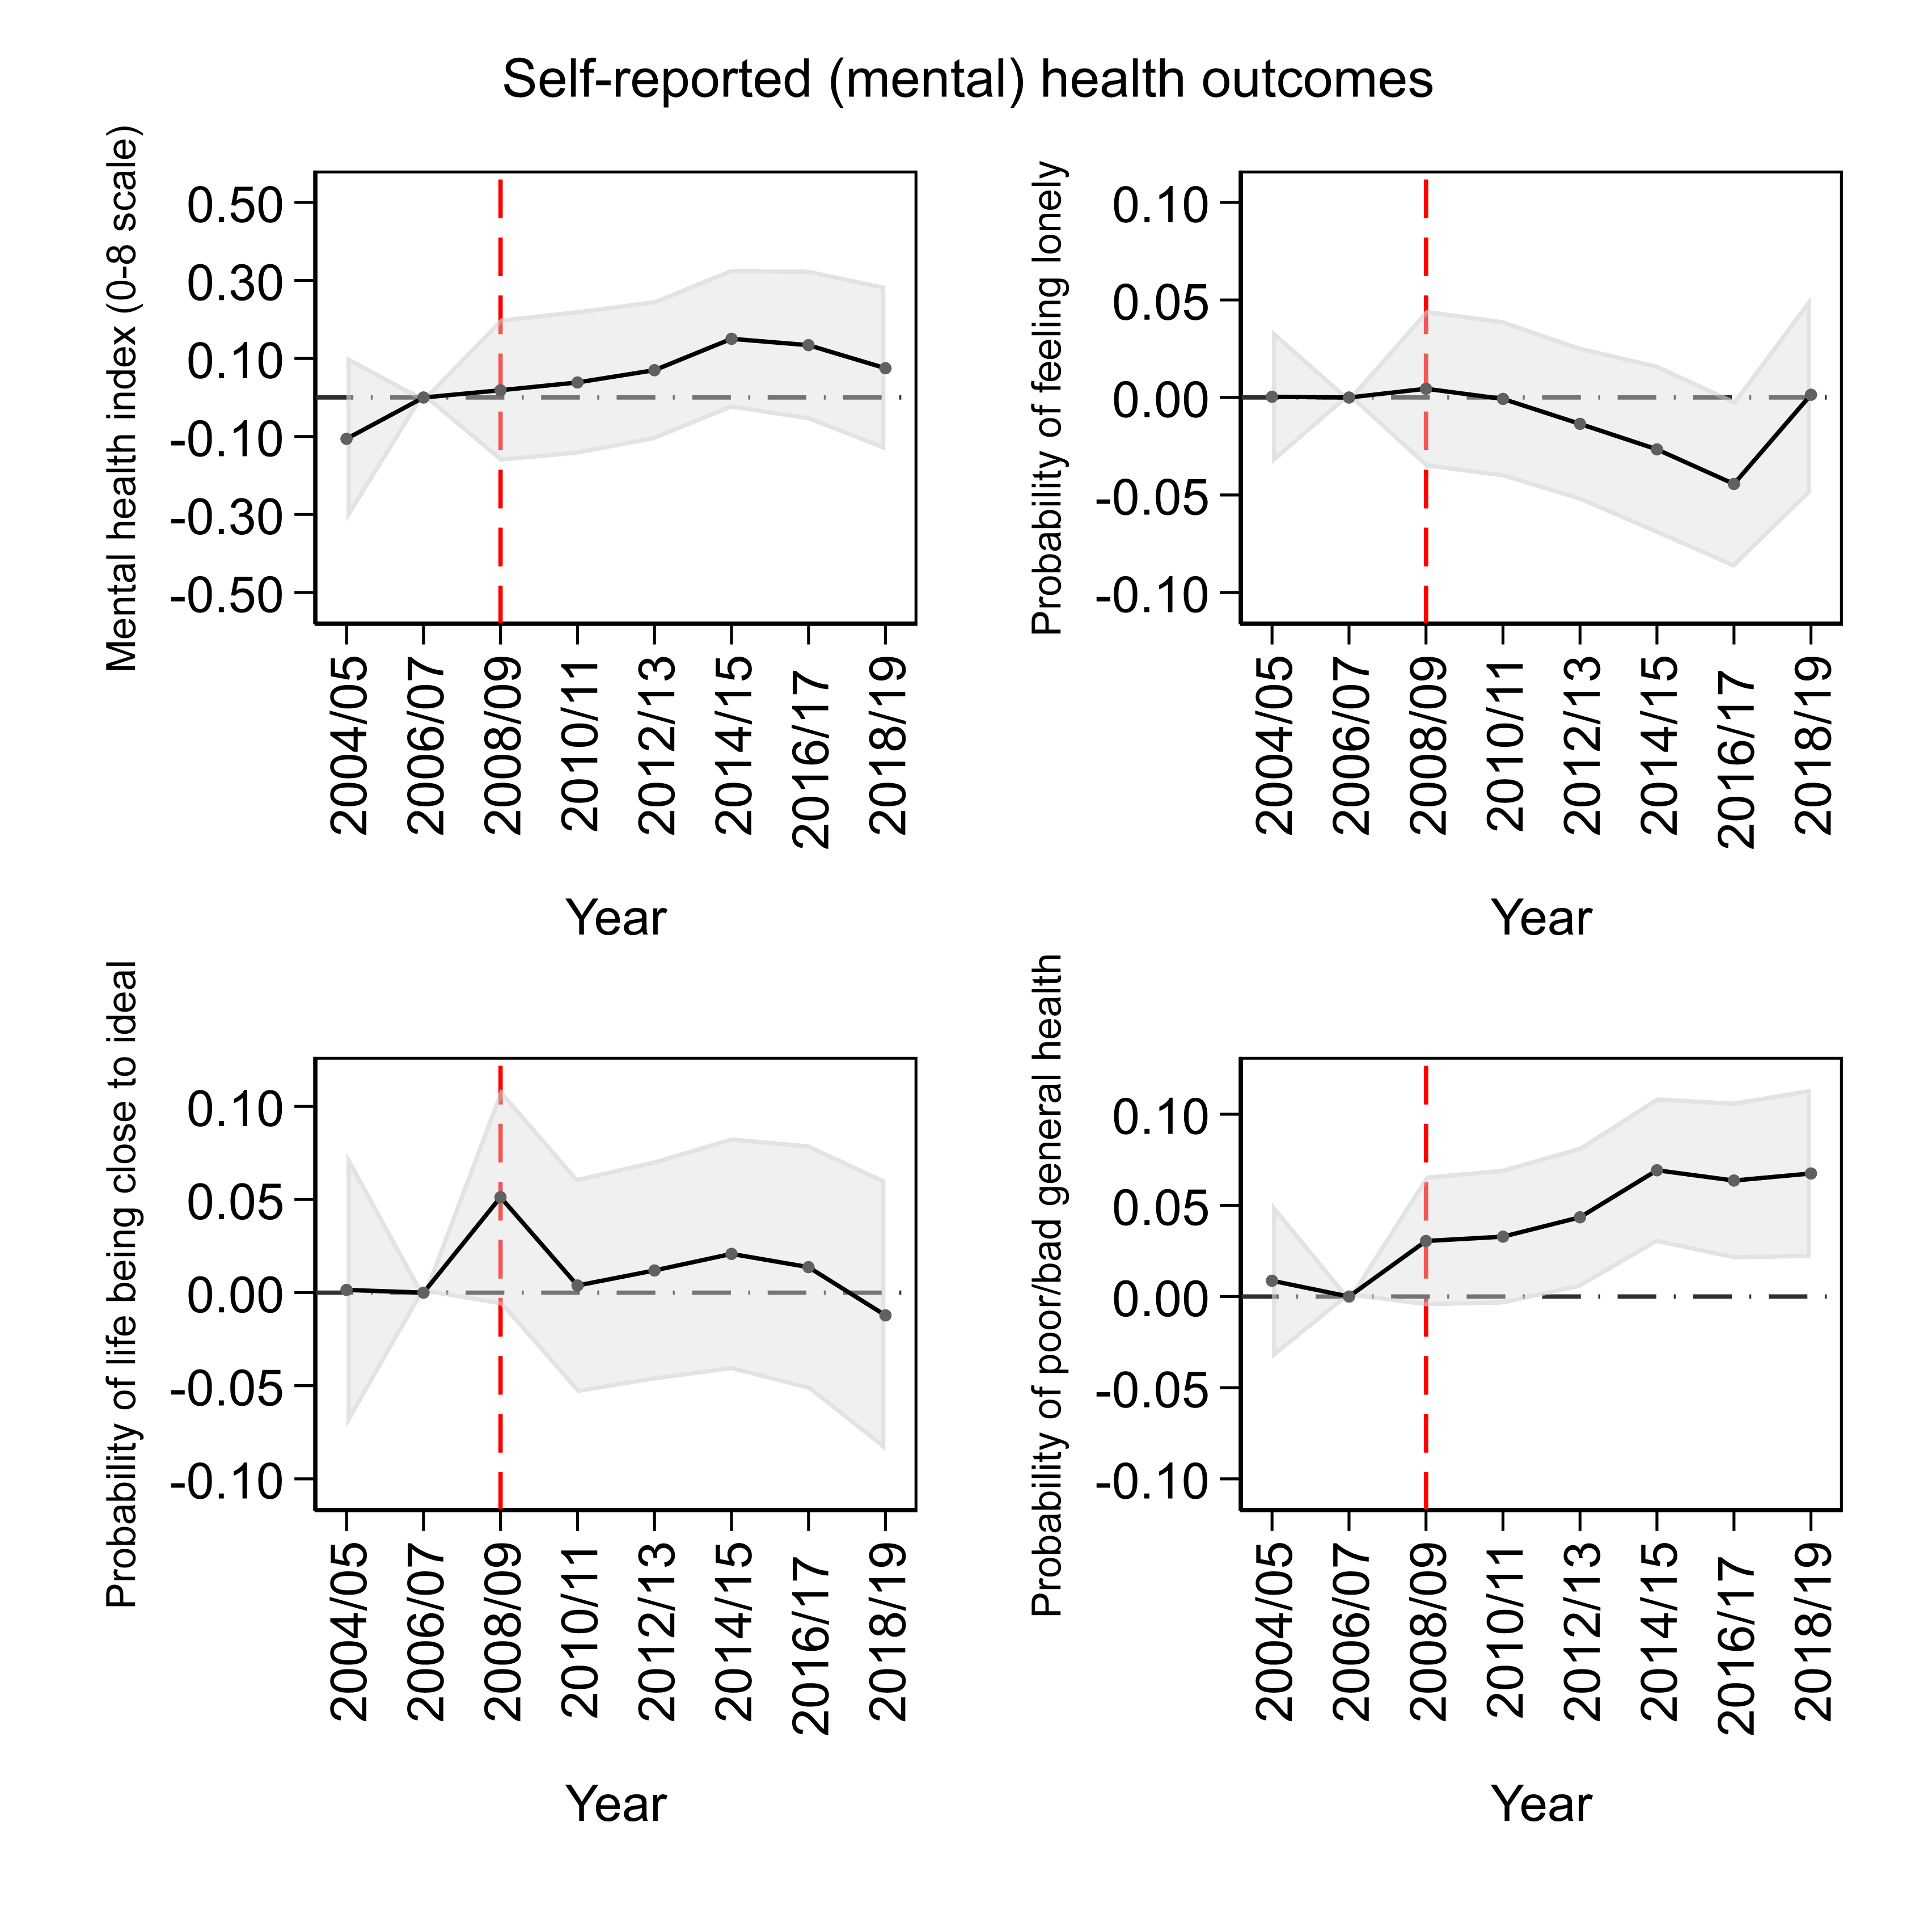
\includegraphics[width=0.86\textwidth]{eventstudy2.png}
\scriptsize{\singlespacing \emph{Notes:} Figure C2 reports the event-study estimates for men for the binary depression indicator and new psychiatric diagnosis.}}
\end{figure}

\newpage
\begin{figure}[htb!]
\caption{Event-study estimates for women}
\label{figC3}
\centering
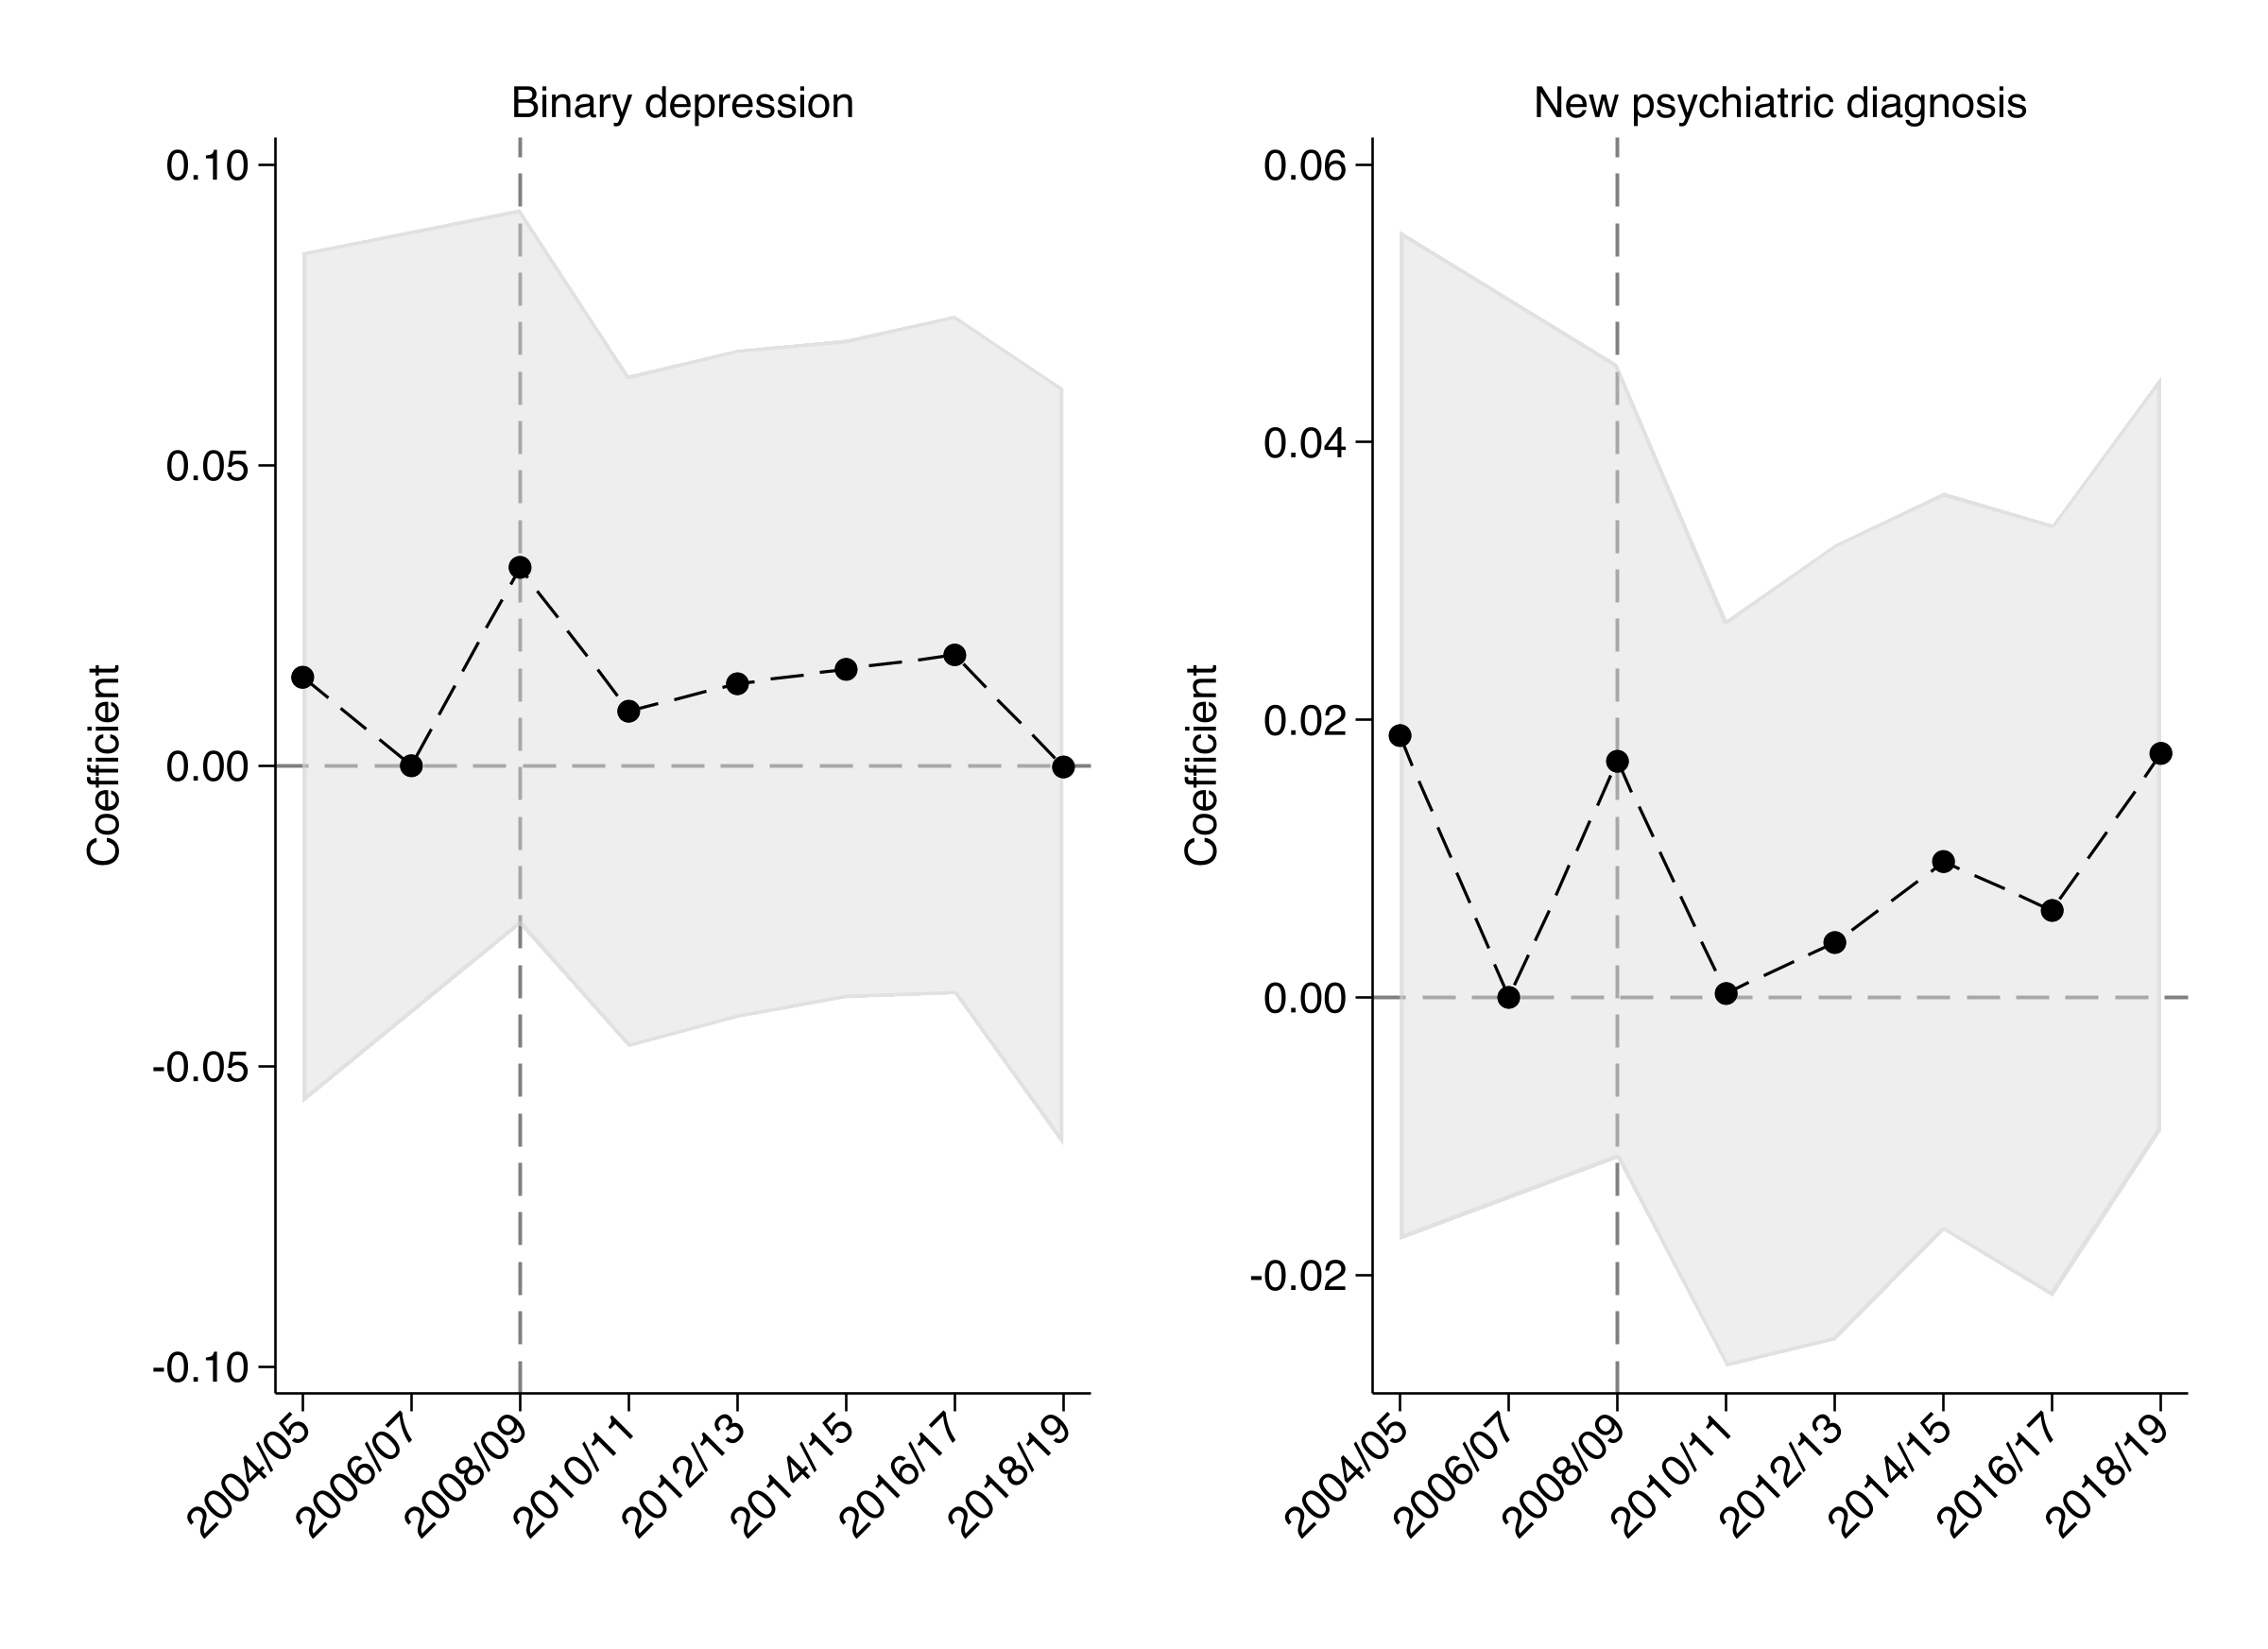
\includegraphics[width=0.90\textwidth]{eventstudy3.png}
\scriptsize{\singlespacing \emph{Notes:} Figure C3 reports the event-study estimates for women for the binary depression indicator and new psychiatric diagnosis.}}
\end{figure}
\end{document}
